\documentclass[
    iict, % Saisir le nom de l'institut rattaché
    il, % Saisir le nom de l'orientation
    %confidential, % Décommentez si le travail est confidentiel
]{heig-tb}

\usepackage{titlesec}

\titleformat{\chapter}[display]
  {\normalfont\bfseries}{}{0pt}{\Huge}

\usepackage[nooldvoltagedirection,european,americaninductors]{circuitikz}
\usepackage{hyperref}
\usepackage{fancyhdr}
\usepackage{lastpage}
\usepackage{pdfpages}
%https://www.overleaf.com/project/62b06d8b8257fff1974999df
%\signature{mbernasconi.svg} TODO : Gérer la taille
\signature{va_signature.png}

\makenomenclature
\makenoidxglossaries
\makeindex

\addbibresource{bibliography.bib}

\usepackage{etoolbox}
\renewcommand\nomgroup[1]{%
  \item[\bfseries
  \ifstrequal{#1}{A}{Constantes physiques}{%
  \ifstrequal{#1}{B}{Groupes}{%
  \ifstrequal{#1}{C}{Autres Symboles}{}}}%
]}

\newcommand{\nomunit}[1]{%
\renewcommand{\nomentryend}{\hspace*{\fill}#1}}

\nomenclature[A, 02]{\(c\)}{\href{https://physics.nist.gov/cgi-bin/cuu/Value?c}
{Vitesse de la lumière dans le vide}
\nomunit{\SI{299792458}{\meter\per\second}}}

\nomenclature[A, 03]{\(h\)}{\href{https://physics.nist.gov/cgi-bin/cuu/Value?h}
{Constante de Planck}
\nomunit{\SI[group-digits=false]{6.62607015e-34}{\joule\per\hertz}}}

\nomenclature[A, 01]{\(G\)}{\href{https://physics.nist.gov/cgi-bin/cuu/Value?bg}
{Constante de gravitation universelle}
\nomunit{\SI[group-digits=false]{6.67430e-11}{\meter\cubed\per\kilogram\per\second\squared}}}

\nomenclature[B, 03]{\(\mathbb{R}\)}{Nombres réels}
\nomenclature[B, 02]{\(\mathbb{C}\)}{Nombres complexes}
\nomenclature[B, 01]{\(\mathbb{H}\)}{Quaternions}

\nomenclature[C]{\(V\)}{Volume constant}
\nomenclature[C]{\(\rho\)}{Indice de frottement sec}

\newacronym{gcd}{GCD}{Plus grand diviseur commun}
\newacronym{lcm}{LCM}{Plus petit multiple commun}
\newacronym{uon}{UON}{Unified Object Notation}
\newacronym{antlr}{ANTLR}{Unified Object Notation}
\newacronym{ebnf}{EBNF}{Extended Backus–Naur Form}

\newglossaryentry{heig-vd}{
    name=HEIG-VD,
    description={Haute École d'Ingénierie et de Gestion du canton de Vaud}
}
\newglossaryentry{hes-so}{
    name=HES-SO,
    description={Haute École Supérieure de Suisse Occidentale}
}
\newglossaryentry{latex}{
    name=latex,
    description={Un langage et un système de composition de documents}
}
\newglossaryentry{maths}{
    name=mathematics,
    description={Les mathematiques sont ce que les mathématiciens fonts}
}
\newglossaryentry{token}{
    name=token,
    description={C'est un segment de texte avec un type associé}
}
\newglossaryentry{grammaire}{
    name=grammaire,
    description={un fichier décrivant formellement un langage}
}
% Auteur du document (étudiant-e) en projet de Bachelor
\author{Vitor Vaz Afonso}

% Activer l'option pour l'accord du féminin dans le texte
\genre{male}

% Titre de votre travail de Bachelor
\title{Support du langage UON sous VS Code}

% Le sous titre est optionnel
\subtitle{Travail de Bachelor}

% Nom du professeur responsable
\teacher {Prof. Y. Chevallier (HEIG-VD)}

% Mettre à jour avec la date de rendu du travail
\date{\today}

% Numéro de TB
\thesis{7212}



\surroundwithmdframed{minted}

%% Début du document
\begin{document}
\selectlanguage{french}
\maketitle
\frontmatter
\clearemptydoublepage

%% Requis par les dispositions générales des travaux de Bachelor
\preamble
\let\cleardoublepage\clearpage
\authentification
\let\cleardoublepage\clearpage

%% Résumé / Version abbrégée
\begin{abstract}
    % Francais

% • le contexte,
En 2018, le professeur Yves Chevallier a imaginé un nouveau format de sérialisation proche de YAML et JSON nommé \Gls{uon}.
UON vise à rassembler toutes les caractéristiques utiles des formats de sérialisation les plus utilisés sur internet (XML, YAML et JSON),
en un seul format qui les englobe. Cela dans le but de le rendre adapté à la communication \Gls{m2m} pour des dispositifs embarqués de faibles puissances, jusqu'aux plateformes haut de gamme basées sur le cloud.

% • la problématique,
Ce Travail de Bachelor a pour objectif de permettre l'utilisation du langage UON dans l'éditeur de code VS Code, en créant une extension disponible depuis le Marketplace de Visual Studio Code.
Cette extension doit fournir à l'utilisateur, le support de langage permettant une meilleure rédaction d'un fichier UON.

Le support est fourni sur une implémentation de la grammaire issue de la spécification UON.
L'API de VS Code est directement contactée pour implémenter les fonctionnalités.
ANTLR est le générateur de parser qui a été choisi.
Le moteur de complétion antlr4-c3 est utilisé comme source principale des suggestions pour l'auto-complétion.

Au terme de ce projet, les points attendus du cahier des charges ont été effectués. Il s'agit de :
\begin{itemize}
    \item Disposer d'une grammaire du langage UON utilisable
    \item Implémenter une intégration continue
    \item Implémenter une coloration syntaxique
    \item Implémenter de l'auto-complétion
    \item Implémenter une outline view
    \item Implémenter l'affichage des informations au survol de la souris (Hover Information)
    \item Implémenter un Linter simple pour signaler des erreurs
\end{itemize}

% • perspectives et recommandations
Les perspectives concernant ce sujet sont vastes, mais des améliorations possibles à ce projet sont les suivants :
\begin{itemize}
    \item Implémenter les points du CDC dans la partie "si le temps le permet".
    \item Utiliser un langage server au lieu de l'API VS Code.
    \item Continuer à améliorer la grammaire et adapter les fonctionnalités en conséquence.
\end{itemize}
\end{abstract}

%% Sommaire et tables
\listoffigures
\addcontentsline{toc}{chapter}{\listfigurename}
\listoflistings
\addcontentsline{toc}{chapter}{Liste des codes sources}

\tableofcontents

\printnomenclature
\clearemptydoublepage
\pagenumbering{arabic}

\pagestyle{fancy}
\fancyhf{}
\renewcommand\headrulewidth{1pt}

\fancyhead[R]{Support du langage UON}
\fancyhead[L]{\itshape\nouppercase{\leftmark}}

\renewcommand{\chaptermark}[1]{\markboth{\MakeUppercase{#1}}{}}

\renewcommand\footrulewidth{1pt}

\fancypagestyle{plain}{%
    \fancyfoot[R]{Page \thepage/\pageref{LastPage}}
}
\fancyfoot[R]{Page \thepage/\pageref{LastPage}}

\renewcommand{\headrulewidth}{0.4pt}
\renewcommand{\footrulewidth}{0.4pt}

\titlespacing*{\chapter}{0pt}{-40pt}{20pt}

%% Contenu
\mainmatter
\chapter{Introduction}

Ce projet de Bachelor consiste à fournir du support pour le nouveau langage de sérialisation UON, sous VS Code.
UON (abréviation de Unified Object Notation) est un format de sérialisation qui vise à rassembler les meilleures caractéristiques de tous les formats de sérialisation disponibles sur le marché, pour créer celui qui les unifie tous.

Ce projet consiste donc à fournir à l'utilisateur, les outils pour lui permettre la rédaction la plus optimale d'un fichier UON dans l'éditeur VS Code.

C'est un nouveau langage complexe et une spécification détaillé existe. Il reste maintenant à construire les éléments permettant son utilisation.

%"Contexte" qui explique comment s'insère ce travail de Bachelor. C'est quoi UON est-ce que quelqu'un a déjà travaillé dessus, ce qu'il a fait, ce qu'il reste à faire.

Un parser en Python à déja été implémenté par Stéphane Selim.
Le travail précédent s'était concentrer sur 3 aspects : La sérialisation/deserialisation binaire et textuelle d'objet en python, la cohércient et la validation.
Cepedendant ce travail de bachelor n'en est pas la suite directe.

Il consite à founir une autre composante qui est de permettre l'utilisation du langage UON dans un éditeur pour qu'il soit utilisé par un plus grand nombre.

Nous nous focaliserons uniquement sur VS code dans un premier temps et expliquerons pourquoi plus tard nous avons choisi cet éditeur.

Ce projet consite à étudier les différentes approches et les mettre en oeuvre. Nous spécifierons également les alternatives et améliorations possible quand cela est pertinent.

Il se veut aussi être expérimental et aussi ouvert à la discussion.
Aucun cadre précis sur sa réalisation n'a été établi et les approches choisies sont libres tant qu'elles respectent le cahier des charges.

Dans les chapitres suivants, nous allons :

\begin{itemize}
    \item Se renseigner concernant ce qui est fourni par VS Code pour élaborer et déployer une extension.
    \item Se renseigner sur les éléments à prendre en compte pour pouvoir fournir du support pour un langage.
    \item Chosir les aspects du langage UON à traiter dans le cadre de ce projet.
    \item Documenter et réaliser l'implémentation d'une extension, son intégration continue ainsi que ses fonctionnalités.
    \item Documenter et mettre en place les tests effectués pour les différents composants du projet.
    \item Documenter également des pistes de réflexions, les alternatives,et améliorations possible.
\end{itemize}

\let\cleardoublepage\clearpage

\chapter{Cahier des charges}
Voici ci-dessous un résumé du cahier des charges :

\textbf{Extension}
\begin{itemize}
    \item Code source publié sur Github
    \item Fournir une intégration continue
    \item Déployer l'extension sur \href{https://marketplace.visualstudio.com/}{le marketplace} de Visual Studio
\end{itemize}

\textbf{Fonctionnalités à implémenter}
\begin{itemize}
    \item Syntax highligting
    \item Auto-complétion
    \item Document Outlining
    \item Hover Information
\end{itemize}

\textbf{Si le temps le permet}
\begin{itemize}
    \item Lint
    \item Formattage : Outil permettant de formatter le code
    \item Converter : Outil permettant de convetir du code
\end{itemize}

\vspace{\parskip}

Concernant les fonctionnalités à implémenter. Il n'y avait pas de contraintes de choix.
Les fonctionnalités choisis ont donc été ceux paraissant être les plus utiles à avoir dans un premier temps, en prenant en considération la contrainte de temps.

Cependant il ne s'agit que d'une infime partie de ce qui peut être réalisable.
Il existe. pour chaque langage, une multitude d'ajouts, d'améliorations possible.

% TODO
On pourrait par exemple mentionner la validation par un schéma...

\chapter{Pré-étude}

\section{Parsing}
Le travail ne portant pas sur cette élément en particulier. Nous n'allons pas rentrer en détail dans ce sujet.
Mais il est important de rappeler les concepts prinicipaux car ces éléments nous sont très utile et il est important de bien en comprendre son fonctionnement.

Afin de pouvoir intérpréter du code, on passe par plusieurs étapes.

La première consite à une analyse lexical à l'aide d'un Lexer. On va décomposer un input (notre code ou texte) en une liste de token.
Ces tokens seront ensuite utiliser lors de l'analyse syntaxique. L'analyse syntaxique consite à regarder quelles sont les règles qui sont applicables pour une suite de tokens défini dans une grammaire.

Le résultat de cette analyse est un "Parse Tree" qui représente toutes les dérivations de notre input en fonction de la grammaire.
Elle est représenté sous forme hiérarchique.

C'est cette strucutre final qui sera intérpté ou compilé.

\begin{figure}[!h]
    \begin{center}
        \frame{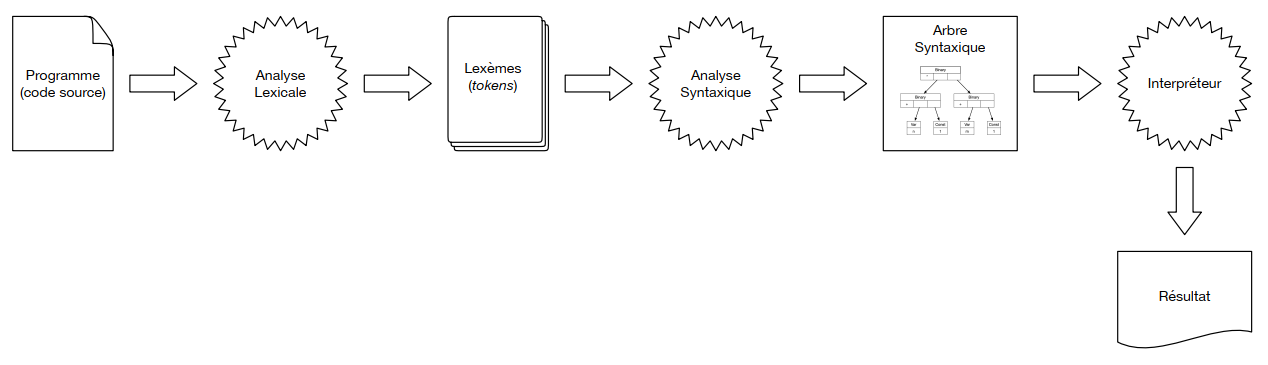
\includegraphics[width=12cm]{assets/figures/interpreter-flow.PNG}}
    \end{center}
    \caption[interpreter-flow Anatomy]{\label{interpreter-flow} interpreter flow}
\end{figure}


\section{Generator de parser}

% https://en.wikipedia.org/wiki/Comparison_of_parser_generators


% TODO
Pour nous simplifier la vie...

% TODO
%  pertinence ? à déplacer dans UON
\section{Format de sérialisation}

% TODO
%%Le code d'un langage de sérialisation dans l'éditeur est "statique".
%Pas de notion de traitement dans un éditeur de code. On ne va appliquer les mêmes traitements quand il s'agit uniquement de UON par rapport à quand il est utilisé avec un langage haut niveau.
%On pourrait créer une extension supplémentaire pour linker le fichier UON au parseur de selim, features + avancé ???

Lorsqu'on sérialise des données, elles se retouvent soit sous forme binaire ou textuelle.

Ce projet se focalisera naturellement uniquement sur le format textuelle car c'est le format que l'on manipulera dans un éditeur.

Le rôle d'un format de sérialsiation et de pouvoir représenté des données sous une autre forme et comprise et intérprétable...

Dans un éditeur de texte c'est statique.

Expliquer le mécanimse. ou c'est utilisé et pourquoi ?

\subsection{JSON}
clé-valeur
\subsection{YAML}
indentation
\subsection{Protobuf}


% TODO
% pourquoi VS Code est pas un autre éditeur ??
% Présenter les autres éditeur de code (atom...)
% C'était l'éditeur proposé mais pas que...
% Popularité, usage personnelle...
% c'est quoi un éditeur de code / rapport avec un Ide / Les difflérences que l'on pourrait avoir
% Que propose les concurents ?

\section{VS Code}
% TODO :
% Peut être élaborer un peu plus : c'est quoi VS Code, pourquoi a-t-il été choisi ? Est-il populaire ? En quel langage a-t-il été écrit. Est-il entièrement open-source, est-ce qu'une extension peut être complètement indépendante de la base de code...
% Pour le rapport final j'attends plus de détails

Il a été choisi car il fait parti des éditeurs les plus populaires. C'est également l'éditeur que j'utilise le plus personnellement et donc je suis déja familier de son environement.
D'autres alternatives existes comme VIM et Atom pour ne citer qu'eux. Et chacun d'eux fourni également de quoi implémenter une extension.
C'est donc un choix personnel. Mais les concepts entre éditeur semble relativement similaire.

L'idéal serait de pouvoir créer un support pouvant être utilisé sur n'importe quels éditeurs. Mais cela n'est pas possible pour plusieurs raisons.
Des fonctionnalités ne peuvent être implémenté que sur un éditeur spécifique. Par ex % todo


Comme il est pensé pour être étendu, il fourni et détaille très clairement les étapes pour la création d'une extension ainsi que le support de langage en lui-même.
La communauté est très active.
De nombreux exemples officieles et d'utilisateurs existents.

Le code source de vscode de Microsoft estopen source (sous licence MIT) mais...

Une extension peut être écrite en Typescript ou en Javascript.
Nous choisirons le Typescript car VS Code recommande ce langage.

Mais certaines composantes externes (langage server) peuvent être écrit dans n'importe quel langage. Tant qu'elle fournisse l'API adéquat pour communiquer.


Visual Studio Code (ou VS Code) est un éditeur de code multi-plateforme, open source et gratuit qui est pensé pour être extensible (de L'UI à l'expérience utilisateur).
Presque tout peut être customisé et amélioré à travers de L'Extension API \cite{extension-api}.


Un éditeur de code est décris selon wikipédia comme un logiciel destiné à la création et l'édition de fichiers textes.
Contrairement à un IDE (Environnement de développement) qui permet en plus la compilation et le debuggage de programme plus complexe.

\textbf{TODO : Faire la distinction de ce qu'on peut faire ou pas dans le cadre d'un éditeur.}

Nous manipulerons des fichiers statiques par la nature même de UON qui est un langage de sérialisation.

Il a été écrit en Typscript et Javascript.

L'Extension API nous permet donc de gérér un certain nombre de choses.
On se focalisera sur le theming, les fonctionnalités de langages, la publication de l'extension et les tests.

VS Code fournit des documentations détaillées sur plein de sujets, des guides, ainsi que des exemples de codes.
Il s'agit donc évidemment de la source principale des explications données dans ce document concernant ce qui touche à cette éditeur.

//TODO : code sample https://github.com/microsoft/VS Code-extension-samples

\subsection{Extension Anatomy}
Il y a 3 concepts cruciaux à comprendre pour réaliser une extension.

\begin{itemize}
    \item \textbf{Activation Events}: Des événements à partir desquels l'extension devient active \cite{activation-events}.
    \item \textbf{Contribution Points}: Des déclarations statiques qui sont faites dans l'Extension Manifest "package.json" pour étendre l'extension. Il s'agit d'un ensemble de déclarations JSON faites au travers du champ "contributes" \cite{contribution-points}.
    \item \textbf{VS Code API}: Un ensemble d'API JavaScript que nous pouvons invoquer dans le code \cite{vs-code-api}.
\end{itemize}

En général, l'extension est une combinaison de plusieurs Conntribution Point et de VS code API pour étendre les fonctionnalités de VS Code.

\subsubsection{Extension File Structure}\label{Extension File Structure}

%TODO : faire figurer un extrait de code / ou faire référence à la figure au lieu de "la suivante"

La structure d'une extension est la suivante :

\begin{figure}[!h]
    \begin{center}
        \frame{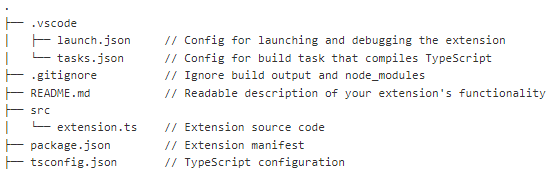
\includegraphics[width=10cm]{assets/figures/extension-anatomy.PNG}}
    \end{center}
    \caption[Extension Anatomy]{\label{extension-anatomy} Extension Anatomy}
\end{figure}

\textbf{Extension Manifest} :
chaque extension doit contenir un fichier "package.json". En plus des champs propres à Node.js, on peut spécifier des scripts, dépendances de développement et des champs spécifiques à VS Code.

\textbf{Extension Entry File} :
il s'agit du fichier prinicipal de l'extension (Extension.js).
De base il contient 2 fonctions : \emph{activate} et \emph{deactivate}.
La fonction activate est executée à l'activation de notre extension par un Activation Event. On initialisera ici notre extension.
La fonction \emph{deactivate} est exécutée lorsque l'application devient inactive et sert principalement à nettoyer le code avant la désactivation de l'extension

\textbf{Remarque} : le niveau de customisation est assez élevé. La seule limitation indiquée et qu'il n'est pas possible d'accéder au DOM de l'éditeur.

Nous avons donc vu les briques de bases pour la conception d'une extension. Mais cette base est suffisante pour commencer à travailler.

Si vous souhaitez vous renseigner d'avantages sur l'élaboration d'une extension vous pouvez consulter la page \href{https://code.visualstudio.com/api}{suivante}.
Concernant les fonctionnalitls générales de l'éditeur VS Code vous pouvez consulter consulter \href{https://code.visualstudio.com/docs}{la documentation officielle}.

\subsection{Support de langage}
VS Code fournit la possibilité d'ajouter du support pour un nouveau langage de programmation au travers d'implémentation de fonctionnalités. Ces fonctionnalités peuvent être classées en 2 catégories détaillées
dans dans les sections \hyperref[Declarative language features][Declarative language features] et \hyperref[Programmatic language features][Programmatic language features] ci-dessous.

\section{Declarative language features}\label{Declarative language features}
Elles ajoutent un support d'édition de texte de base pour un langage de programmation.
Par exemple, les éléments suivants :

\begin{itemize}
    \item syntax highlighting
    \item snippet completion
    \item bracket matching
    \item bracket autoclosing
    \item bracket autosurrounding
    \item comment toggling
    \item auto indentation
    \item folding (by markers)
\end{itemize}

Il s'agit de fonctionnalités implémentées à l'aide de fichier de configuration.

Puis, elles doivent être enregistrées comme \emph{Contribute Point}.

\section{Programmatic language features}\label{Programmatic language features}
Il s'agit de fonctionnalité plus riche et plus complexe à mettre en place (p.ex : "Hovers", "Go to Definition", "diagnostic errors", "IntelliSense" \space et "CodeLens".
Il y a 2 approches pour les implémenter que nous allons voir ci-dessous.

\subsection{VS Code API (Direct implementation)}
La première solution est d'utiliser \href{https://code.visualstudio.com/api/references/vscode-api#languages}{l'api vscode.languages.*}
VS Code fournit sa propre API pour implémenter directement les fonctionnalités du langage.

Elles vont nous permettre de nous inscrire à des providers. L'éditeur de code fera ensuite les requêtes à ces providers lorsque cela sera nécessaire.

%TODO : Pas forcément uniquement des providers (ex suggestions)}

\subsection{Langage server}
La seconde solution est de fournir nous-mêmes ces méthodes en respectant la spécifiation LSP \cite{lsp-specification} au travers d'un langage serveur.
Les avantages souvent mentionnés ce cette approche sont que le langage server peut être écrit avec le langage que l'on souhaite et
que cela permet aussi à d'autres éditeurs de texte compatibles avec le langage server d'utiliser ces fonctionnalités sans devoir les implémenter de nouveau.

Mais comme points négatifs cette approche est plus complexe à implémenter et dans notre cas n'est pas un choix primordial.

Pour être utilisé sur VS Code, un langage server à 2 parties :
\begin{itemize}
    \item \textbf{Un client} : c'est une extension écrite en Javascript ou Typescript qui à accès à tous les endpoints de VS Code.
    \item \textbf{Langage server} : un outil d'analyse linguistique fonctionnant dans un processus séparé.
\end{itemize}

\vspace{\parskip}

Le client et le serveur communiquent à l'aide du protocole LSP (pour "language server") dès que des informations riches devraient être fournies à l'éditeur.
Le langage server devrait ensuite pouvoir "consommer" un parser pour traiter les fonctionnalités. C'est-à-dire être capable d'analyser un AST et de fournir une réponse adéquate.
L'implémentation d'un tel serveur peut être libre, mais des implémentations existent déjà. Telle que "LSP4" implémenté en Java ou  "VS Code-languageserver-node" implémenté en Typescript qui n'est pas exclusivement réservé à VS Code comme son nom pourrait l'indiquer.
On remarque donc avec cette approche que deux composantes existent (le client et le serveur).
Un langage server peut être utilisé sur d'autre éditeur compatible. Mais le client devra être implémenté de nouveau.

% TODO
On pourrait vite se réjouir est pensé que n'importe quelle éditeur ou IDE \dots

"NOTE: The first time I read about LSP I thought (naively) that any editor or IDE with LSP support could simply connect to any LSP language server. 
This is not the case: most non-trivial LSP servers require each editor to also have a language-specific (even if small) LSP client. 
The main responsibility of each LSP client is to launch the server, and then pass on the connection information to the editor/IDE."



\subsection{API vs LSP}\label{api vs lsp}

Le schéma suivant \ref{api vs lsp} montre la correspondance des méthodes entre la première et seconde approche.
Cette liste est non exhaustive, mais permet de montrer l'équivalence des 2 méthodes.

\begin{figure}[!ht]
    \begin{center}
        \frame{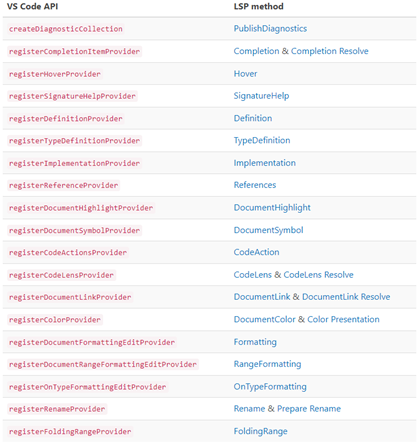
\includegraphics[width=8cm]{assets/figures/api-vscode.png}}
    \end{center}
    \caption[API vs LSP]{\label{api vs lsp} VS Code API vs LSP method}
\end{figure}

\subsection{Parser}
Pour fournir des fonctionnalités de langue, une approche souvent mentionnée est l'utilisation d'un parser
car les fonctionnalités se baseront sur l'AST qu'il générera.

%TODO : être plus clair
Cependant dans le cadre de son utilisation dans un éditeur ou IDE, il devrait être "fault tolerant". Le parseur doit pouvoir générer un AST (abstract syntax tree) qui à du sens depuis du code incomplet
car il ne devrait pas s'arrêter dès la première erreur.
La plupart du temps, le code dans l'éditeur est incomplet et syntaxiquement incorrect, et les développeurs s'attendent tout de même à ce que la complétion automatique et d'autres fonctions de langue fonctionnent.

\subsection{Grammaire}
Il faudra aussi élaborer une grammaire pour le langage de sérialisation UON utilisable par le parser.
Pour faciliter l'étape de l'analyse syntaxique ("Parsing"), cette grammaire pourrait être plus permissive, en particulier concernant les types attendus (Terminaux).
Ainsi si l'utilisateur entre une valeur dont le type attendu est incorrect (par rapport aux spécifications du langage). Nous n'avons pas à traiter ce type d'erreur.

% Différente catégorie de grammaire (nous la 2 ?)

\section{Choix technologiques}
Nous allons mentionner les technologies et approches choisies et expliquer les raisons.

\subsection{Direct implementation}
L'implémentation d'un langage serveur n'étant pas une priorité et pour se concentrer sur la réalisation des fonctionnalités, l'approche de contacter directement l'api de VS Code sera choisi.
Si le temps le permet, toute la logique du code concernant les fonctionnalités pourrait être déplacée dans un langage server.

Beaucoup de possibilités existent comme mentionné au point \hyperref[api vs lsp]{API vs LSP}, mais nous utiliserons uniquement les providers suivants :

\begin{itemize}
    \item \textbf{registerCompletionItemProvider} : Pour afficher des suggestions de complétions.
    \item \textbf{registerHoverProvider} : Pour gérer le hover.
    \item \textbf{registerDocumentSymbolProvider} : Pour afficher les éléments dans la Outline View.
\end{itemize}

\subsection{ANTLR}

%TODO : Détailler en détail l'histoire d'antlr...etc...
%    A l'origine en java, une implémentation en typescript existent
%    Pourquoi prévilégier celui-ci et pas un autre
%    Liste des parseur de générateur existant


%TODO : Bien mentionner que l'on va utiliser antlrts et pas sa version en java}
%TODO : Détailler antrlts ? (Les erreurs etc... dans auto-completion ?)}
%TODO : Gérer les commentaires lors du parsing (analyse syntaxique)}
%TODO : gérer correctement les erreurs. On devrait pourvoir continuer le plus possible, actuellement ça bloque la suite ?
%    expliquer les fonctions / ErrorListener
%    A voir https://stackoverflow.com/questions/26675254/antlr-error-strategy-to-skip-tokens-until-rule-matches-again

% TODO
\textbf{Debugging}
JAVA - vaut pas trop la peine de détailler
Affichage Vscode (arbre mais sans strucutre)
Outil pour voir les ATN (plugin vscode)
Intelej plugin
fonction antl4-c3


Il s'agit d'un générateur de parseur, il est actuellement dans sa quatrième version.

Il a été créé par Terence Parr à l'Université de San Francisco.

Il est très utilisé, autant dans le monde académique que profesionnel.

L'algorithme de parsing utilisé dans sa version la plus récente est le "Adaptive LL(*)" qui est décrit comme amélioration de l'algorithme
"LL(*)" utilisé dans ssa version précédente.

% https://en.wikipedia.org/wiki/LL_parser
% https://www.antlr.org/papers/allstar-techreport.pdf

Dans les grandes lignes  % TODO %

Depuis une grammaire, qui est un fichier décrivant formellement le langage, ANTLR génère le code perméttant de reconnaitre ce langage.
C'est à dire en pratique un lexer et un parser.

La grammaire est décrite en utilisant la notation EBNF (Extended Backus–Naur Form).

Le parser peut automatiquement créer un "parse tree" qui est une structure représentant comment la grammaire interpète un input.
ANTLR peut génèrer également automatiquement un "tree walkers" qui nous permet de visiter chaque noeud de l'abre pour y exécuter des actions liés à notre application.
%TODO : citer antlr.org et wikipedia ?
% https://www.antlr.org/about.html
% https://en.wikipedia.org/wiki/ANTLR

Il n'y a seulement qu'un seul outil qui permet de générer le code des lexer et parsers pour tous les langages cibles, et il est écrit en Java.

Pour pouvoir utiliser cet outil dans un environnement autre que java, il est nécessaire de l'utiliser dans un runtime (environnement d'éxécution) propre au langage shouhaité.
%TODO : citer target.md de antlr et repo antlr4ts ?

% TODO : liens + emph ?

% fork du répo principal antl ?
Nous utiliserons antlr4ts, qui est un environement d'éxécution en typescript et donc parfaitement adapté pour VS Code.

Il a été conçu par l'organisation principalement par Sam Harwell indépendamment de l'organisation ANTLR.
L'organisation ANTLR ne proposant pas de runtime en typescript. %lien ? ou citation
% https://github.com/antlr/antlr4/blob/master/doc/targets.md
% https://github.com/tunnelvisionlabs/antlr4/blob/master/doc/targets.md

% https://github.com/sharwell
% https://github.com/tunnelvisionlabs

% lecture
%https://stackoverflow.com/questions/41427905/how-many-ways-are-there-to-build-a-parser

Cette implémentation semble très apprécié et utilisé.

La raison principal d'utiliser parseur est de pouvoir exploiter un arbre contenant la structure du document.
On pourrait se demander s'il est possible de se passer d'une telle strucutre et de n'utiliser à la place uniquement des expression régulières.
Cependant un problème majeur survient rapidement si on choisit cette approche, la récursivité devient extrèment difficle à traiter.

"you cannot find a (regular) expression inside another one, unless you code it by hand for each level. Something that quickly became unmaintainable."

Example : % TODO

Lorsque que la grammaire a été défini, on peut demander à antlr de générer des parsers dans différents langages.

ANTLR est composé de 2 parties principales : L'outil en java qui permet de générer le lexer et le parseur, aisni que l'environnement d'éxecution (runtime) qui permet leur exécution

%The tool will be needed just by you, the language engineer, while the runtime will be included in the final software created by you.
%Typical Workflow


\subsubsection{Parser}
Étant donné que ce n'est pas le sujet de ce Travail de Bachelor, il a été choisi d'utiliser un générateur de parser pour en extraire le plus possible de complexité sur son implémentation.

Des outils permettant la génération d'un parser existent à partir d'une grammaire.
J'ai opté pour le générateur d'ANTLR (ANother Tool for Language Recognition), car :

% use ANTLR 4 for parsing tasks inside of a TypeScript application
% tree-sitter ????
\begin{itemize}
    \item C'est un outil populaire est encore utilisé.
    \item Il est disponible directement en Typescript \cite{antlr4ts}.
    \item Un moteur de complétion existe avec les parser générés avec antlr. Nous simplifions de grandes étapes pour implémenter l'auto-complétion \cite{antlr4-c3}.
    \item Quelques exemples existent d'implémentation.
    \item La génération est simple.
\end{itemize}

\textbf{Remarque} :
Comme mentionné plus loin au chapitre \hyperref[grammar scope]{4}. Le précédent travail de Bachelor s'était concentré sur l'utilisation d'un parseur généré depuis une spécifiation Lark.
L'implémentation de son parser n'a pas été privilégié car il aurait été nécessaire de créer l'infrastructure permettant de l'utiliser.
Et Antlr semble être un choix plus naturel dans notre environnement VS Code.
%TODO : Founir une meilleur explication

\section{UON}
UON est essentiellement un langage de sérialisation qui est un superset de JSON et un superset partiel de YAML.
Il cherche à regrouper les meilleures caractéristiques de ces formats de sérialisation en un seul format.
Il fournit également des fonctionnalités supplémentaires utiles pour augmenter l'interopérabilité entre différents types de dispositifs, valider les données ainsi que pour diminuer le payload.

Nous allons voir ci-dessous un aperçu général de ce langage.

\subsection{Pourquoi ?}
Son rôle est d'être utilisé dans l'industrie 4.0. Plus particulièrement dans la communication m2m (machine to machine) ainsi que pour l'IoT (Internet of Things).
Ces communications nécessitent souvent de communiquer entre de petits appareils dont la puissance de calcul est très limitée.
La perspective de disposer d'un protocole de communication applicatif à la fois interopérable et adapté aux échanges à faible puissance est très appréciable.
Parce que \textbf{TODO....}

\subsection{Communication}
Lorsque deux appareils veulent échanger des informations, ils disposent de deux canaux de communication :
\begin{itemize}
    \item Un canal de communication en ligne utilisé pour la transmission des données de contenu (payload). Les données peuvent être représentées sous forme humaine et binaire.
    \item Un canal de communication contractuel utilisé pour l'accord sur la description des données (schema).
\end{itemize}

\vspace{\parskip}

À la figure \ref*{data-exchange}, on a à gauche deux dispositifs : un capteur de température à faible consommation
et une puissante passerelle domotique. Pour réduire la taille du payload, les deux dispositifs peuvent convenir d'un schéma qui décrit le format des données.

\begin{figure}[!h]
    \begin{center}
        \frame{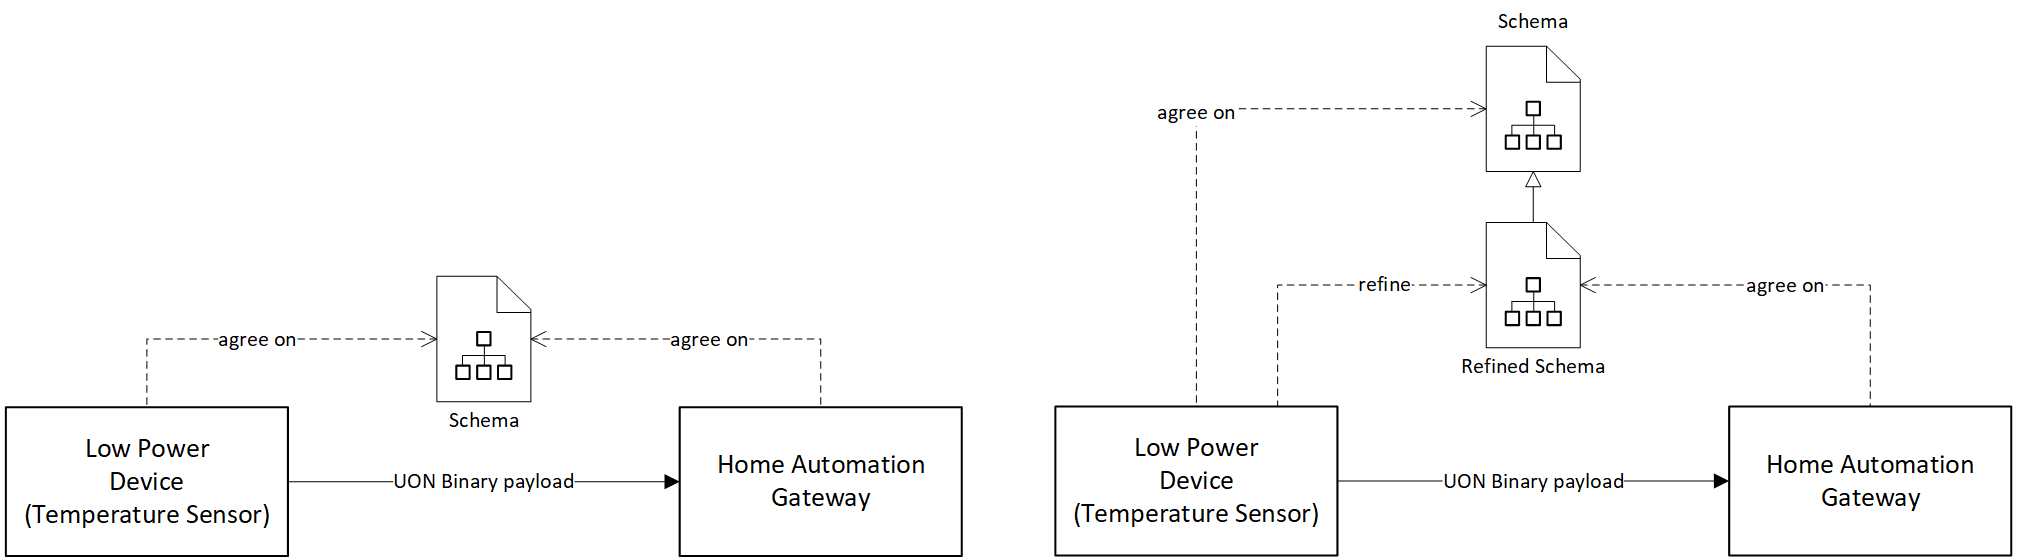
\includegraphics[width=15cm]{assets/figures/data-exchange.png}}
    \end{center}
    \caption[UON data exchange]{\label{data-exchange}UON data exchange}
\end{figure}

À droite on affine le schéma. Pour réduire davantage les données transmises.
Par exemple, en disant que la température exprimée avec un nombre est maintenant une valeur non signée de huit bits exprimée en degrés Celsius.

\subsection{Design}
UON est complètement conforme avec JSON et partiellement avec YAML.

Il peut être décomposé au travers de 4 niveaux de complexités :
\begin{itemize}
    \item \textbf{UON:0} est entièrement compatible avec JSON en ce qui concerne le RFC8259.
    \item \textbf{UON:1} est partiellement conforme à YAML.
    \item \textbf{UON:2} fournit des propriétés de type, la coercition et les chaînes de caractères multilignes.
    \item \textbf{UON:3} offre des types et des références riches.
\end{itemize}

\subsection{Types}
Chaque élément est composé d'un type. Et chacun de ces types peut avoir des propriétés.
3 types de propriétés existent :
\begin{itemize}
    \item \textbf{Presentation properties} : Elles influencent la présentation d'une valeur.
    \item \textbf{Validation propeties} : Elles sont utilisés pour valider, contraindre et décrire un fichier UON.
    \item \textbf{Application properties} : Elles ne peuvent être lues que depuis UON en utilisant le type !prop. Elles sont accessibles depuis l'application (Python, JavaScript, ...). Elles sont utilisées pour générer un fichier sérialisé (binaire, ou UON), mais elles ne sont jamais explicitement transmises.
\end{itemize}

\subsection{Validation}
Dans de telles communications, la validation des données transmises entre des machines dont la puissance de calcul est très limitée est un atout majeur.
Une des propriétés uniques de UON est l'usage de schéma directement intégré dans le langage.

\subsection{Liens}
Si vous souhaitez vous renseigner d'avantages, la spécification complète du projet se trouve sur cette \href{https://github.com/uon-language/specification/}{page}.
Et le dépôt du projet se trouve \href{https://github.com/uon-language/specification}{ici}.

\textbf{TODO : Datatypes ?}

\subsection{Quoi traiter ?}
Il est important d'avoir une bonne compréhension de ce que le langage propose afin de fournir un support pertinent.
Uon est un langage comprenant plusieurs composantes est particulatités qui ne peuvent pas tous être traiter dans un simple éditeur de texte.
La cohercien....

D'autres sont relativement approprié

Tout est une valeur avec un type et des propriétés associés. Ces propriétés sont parfois unique.


\chapter{Scope de la grammaire}\label{grammar scope}
Pour pouvoir proposer du support pour un nouveau langage, il est nécessaire de savoir sur quoi celui-ci portera. Il est donc important préciser sur quels éléments du langage (grammaire) nous nous focaliserons.
Nous allons donc partir d'une grammaire la plus minimale possible tout en faisant attention à son extensibilité par la suite.
Cette grammaire se trouve dans le fichier UON.g4.

Elle est une adaptation de la grammaire écrite en Lark par l'ancien élève Stéphane Selim pour son travail de bachelor "Parser for a serialization language UON". Son travail se trouve sur :
\href{https://github.com/uon-language/uon-parser}{https://github.com/uon-language/uon-parser}

Elle sera complétée et améliorée après la mise en place des fonctionnalités attendues, si le temps le permet.

Les fonctionnalités implémentées s'appuieront sur cette grammaire. Ceci dans le but de rester cohérents entre eux.

\textbf{Rappel} :
La grammaire actuelle nous permet de définir des maps, séquences dans le format json et yaml. D'ajouter des propriétés à des types et également la possibilité de définir un schéma pour un type custom.
% TODO : 3 embranchements différents -> Json(seq et map), Yaml(seq et map) et schema. Donc pas possible de combiner du yaml avec du json

\section{Modification}
% TODO : expliquer la strucutre du fichier json5.g4 que j'ai adapté. Car il conntenait les regex pour gérer les string de manière souple
% TODO : ajouter la gestion des indent pour les sequences en version yaml
% TODO : rajouter ce qui manque dans la grammaire (minus,plus etc...) + faire attention aux erreurs de saisies
% DONE : Gestion des INDENT ET DEDENT (Modification de la grammaire ?), + explication (parti avec grammaire sans la gestion des espaces....)
% TODO : gérer erreur grammaire -> caractère qui bloque le parsing, des erreurs devraient être générés à la place , erreur avec "name", "parameters"
% TODO : visualisation graphique de l'arbre (java ou extension intellij)
% TODO : utiliser les types correctes ou avoir 2 grammaires différentes et donc 2 parsers en paralleles ?
% TODO : autocomplétion dans les commentaires ?
% TODO : expliquer les règles : https://github.com/antlr/antlr4/blob/master/doc/grammars.md
% TODO : règle Clé
% @members -> injection code
% regex pas possible genre ^ symbole ...
% fragments: they are reusable building blocks for lexer rules.
% Error tolerance: This can partly be resolved by making the grammar itself more error tolerant and solving those errors later. -> https://github.com/lark-parser/lark/issues/684 


% Rajout d'unités
% Rajout de propriétés au types (présentation) directement dans le payload
% Rajout des validation propriétés dans un schéma
% Remettre le yaml ??

% Bug : Resolu en créant un lexer token pour les mots et l'utiliser dans le parser rule "string"
% Le truc avec UON c'est qu'on a plein de mon clé. Mais on aussi envie de les utilisers parfois dans les clés
% Si on crée un nouveau token (le fait automatiquemnt meme si on fait jusqze qu écrire du texte) alors il faudra le spécifier dans les clé sinon erreur !!!!



\subsection{L'indentation}

% TODO : Détailler en détail la réflexion ci-dessous
Après refléxion, la gestion des indentations n'a pas été implémentée. Cependant, il est intéressant de détailler son implémentation dans un environnement ANTLR
et plus particulièrement typescript.

L'idée de gérer l'indentation venait du fait que le UON est décrit comme un set partielle de YAML\dots

Pourquoi ? Yaml compliant... / être au plus proche de la specs
Ne pas séparpillier...

On veut éviter au maximum la confusion sur ce qui est possible de faire (ex yaml avec les sequence ? que le prof m'a montré)
Les indentations complexifie énormément dans une contexte (JSON et schéma)
Parler de l'envie exploratoire
Grammaire reprise mais du coup sera réadapté
%%%%%

Contrairement au parser lark, la gestion des indentations n'est pas géré automatiquement à l'aide d'une librairie externe.
Ce méchanisme doit malheurseuement être traité par nos soins.

La grande modularité d'ANTLR est un avantage mais peu se revéler très contraignant pour ce genres de tâches.

Mais avant de résoudre ce problème, il est nécessaire de rappeler que notre grammaire n'est pas uniforme concernant la gestion des retours à la ligne.

En effet, UON peut-être écrit sous une forme proche de JSON ou de YAML. Le premier ne tient pas compte des indentations contrairement à la seconde.

Et la gestion des indentations nécessite de prendre en compte les retour à la ligne. % TODO newline regex

Il y a donc trois solutions qui ont été envisagées.

La première est de rajouter des token de retour à la ligne partout ou il serait possible d'en avoir. Mais ce n'est pas très propre et on risque d'en placer énormément.
Le problème et que dans le cas du format proche de JSON, il faudrait traiter énormément de cas pour rester cohérent.

Le deuxième serait d'ignorer tout simplement les erreurs. C'est à dire que si on à un token de retour à la ligne qui ne devrait pas être là, alors l'ignorer tout simplement.
On pourrait penser ce mécanisme simple se révelerait efficace. Cependant je n'ai malheurseuement pas réussi à faire que le moteur de complétion c3 \textbf{TODO : ICI}
puisse ignorer ces erreurs.

La troisième solution trouvée et celle actuellement utilisée. Elle consite à prendre en compte uniquement les retours à la ligne si le lexer à détecter les tokens initiaux
nous permettant de savoir si oui ou non les retours à la ligne doivent être pris en compte.

Par exemple, tester que le premier token est un token de type MINUS ("-"). On peut déduire qu'il s'agira d'une séquence en format yaml. % TODO

Dès lors que les retours à la ligne existe, nous pouvons maintenant placer les tokens INDENT et DEDENT nécessaire dans le lexer
pour pouvoir gérer les imbrications correctement.

Pour ce faire, à chaque fois qu'un espace qu'un retour à la ligne est detécté, nous prenons compte de la taille de l'espacemment qu'il contient ("\\r\\n    ")
Cet espacement nous permettra de savoir si l'on doit rajouter des INDENT ou DEDENT.

% À chaque fois que le lexer detecte un token on regarde le suivant. Si c'est un retour à la ligne on va appliquer un traitement spécifique
% TODO : More explications -> nextToken , @members, fonction pour ajouter INDENT et DEDENT etc...

\begin{lstlisting}[frame=single,caption={generator-code},label={generator-code}]
    yaml_seq : INDENT (SEQUENCE_TYPE)? seq_item+ DEDENT;
\end{lstlisting}

Pour créer les tokens INDENT et DEDENT


\textbf{Remarque : } Mais cette solution n'est pas optimale car si on modifie la grammaire il faudra probabement modifier ce code.

%Il faut prendre en compte les retours à la ligne.
\subsection{Token DEDENT et INDENT}
Ces deux tokens sont ajoutés depuis le lexer. Cela nécessite d'y rajouter le code pour le faire.

% TODO mieux...
On peut le faire depuis la grammaire. Il suffit d'écrire le code permettant de le faire à l'intérieur de @lexer:members{}.
Lors de la génération, ce code sera déplacé dans le lexer.
Mais j'ai constaté quelques bugs, probablement du au faites que cette implémentation en typescript et récente et que tout n'a pas été pris en compte.
Par exemple il est nécessaire après coup de corriger ce fichier en y rajoutant les imports manquants.

% TODO
\subsection{Règles ?}
Une règle doit suivre le pattern suvant : NEWLINE DEDENT [RULE] INDENT

\chapter{Implémentation}
Dans ce chapitre, nous allons explorer les aspects techniques concernant l'implémentation de fonctionnalités. Nous allons voir également plus en détail les outils utilisés ainsi que le déploiement de l'extension sur le marketplace.
Ce travail reflète uniquement mon approche personnelle sur la matière. Et ne devrait pas être considérée comme l'unique manière de procéder.

% TODO : Taux "d'erreur" acceptable pour le rendu final ?
\section{Tolérance}

"The parser should only check the syntax. So the rule of thumb is that when in doubt you 
let the parser pass the content up to your program. Then, in your program, you check the semantics and make sure that the rule actually have a proper meaning."
% Citation !!!


Le parseur doit pouvoir traiter un fichier correct
Mais si trop correct il y a potentiellement + d'erreurs qui peuvents être detecté

La gestion des erreurs se fait à l'aide des fichiers de stratégies.

Mais on ne peut pas imaginer ignorer / modifier tout correctement\dots


\section{Code}
% TODO : mettre à jour le readme
Le code de l'implémentation est disponible sur le dépôt public \href{https://github.com/vitorva/vscode-uon}{suivant}.

\textbf{Remarque} : L'implémentation détaillée dans ce rapport pourrait ne plus représenter l'état du dépôt, car ce projet est sujet à évoluer.

\section{Extension}
Nous allons voir maintenant, la procédure pour créer et publier son extension.

% TODO : Expliquer que c'est une procédure minimaliste, les explications détaillés sur la documentation vs code

\subsection{Génération de l'extension}
% TODO : expliquer qu'est-ce que Yeoman

VS Code permet de générer un squelette (boilerplate) pour la réalisation d'une extension. Pour ce faire il faut avoir Node.js et Git installés, pour installer Yeoman et VS Code Extension Generator avec la commande :

% TODO : yeoman Generator to scaffold an extension...

\begin{lstlisting}[frame=single,caption={generator-code},label={generator-code}]
npm install -g yo generator-code
\end{lstlisting}

Puis il suffit de saisir la commande :

\begin{lstlisting}[frame=single]
yo code
\end{lstlisting}

et de compléter ce qui est attendu dans le terminal.

\begin{figure}[!h]
    \begin{center}
        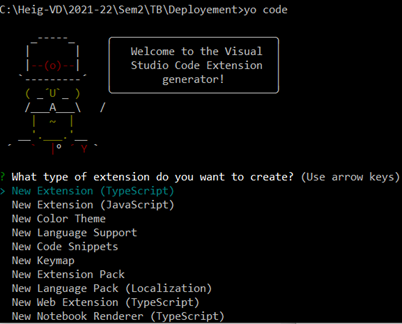
\includegraphics[width=8cm]{assets/figures/yo-code.png}
    \end{center}
    \caption[Yo Code generator]{\label{yo-code}Yo Code generator}
\end{figure}

Cela nous créera l'arborescence mentionnée précédemment au point \hyperref[Extension File Structure]{Extension File Structure}.

\subsection{Lancement de l'extension en debug}
On peut lancer une nouvelle fenêtre (f5) qui va contenir notre extension.

Par défaut, l'application générée vient avec du code permettant d'afficher un message de bienvenu. On l'affiche au travers du command pannel (CTRL + SHIFT + P). On peut s'assurer comme cela que l'implémentation de base fonctionne correctement.
On constate donc que l'on peut lancer notre application au travers d'une commande, mais pour notre cas il sera plus intéressant que VS Code nous propose les fonctionnalités à l'ouverture d'un fichier uon.
Pour cela, il faut modifier l'activation events dans le fichier package.json par :
\begin{lstlisting}[frame=single]
    "activateEvents" : [
	"onLanguage:uon"
    ]
\end{lstlisting}

\subsection{Déploiement sur le Marketplace}

% https://code.visualstudio.com/api/working-with-extensions/publishing-extension
% https://code.visualstudio.com/api/working-with-extensions/continuous-integration
% https://marketplace.visualstudio.com/manage/publishers/test2publish?noPrompt=true
% https://dev.azure.com/Stev03/_usersSettings/tokens

\textbf{Prérequis} : Posséder un compte Azure.

% En gros on va créer un acces TOKEN depuis notre compte qui nous permettre d'avoir les droits pour publier une extension

Il faut d'abord récupérer un Personal Access Token. Pour ce faire, il faut créer une \href{https://docs.microsoft.com/en-us/azure/devops/organizations/accounts/create-organization?view=azure-devops}{organisation}.
Puis, créer un access token avec ces paramètres :
\begin{figure}[!h]
    \begin{center}
        \frame{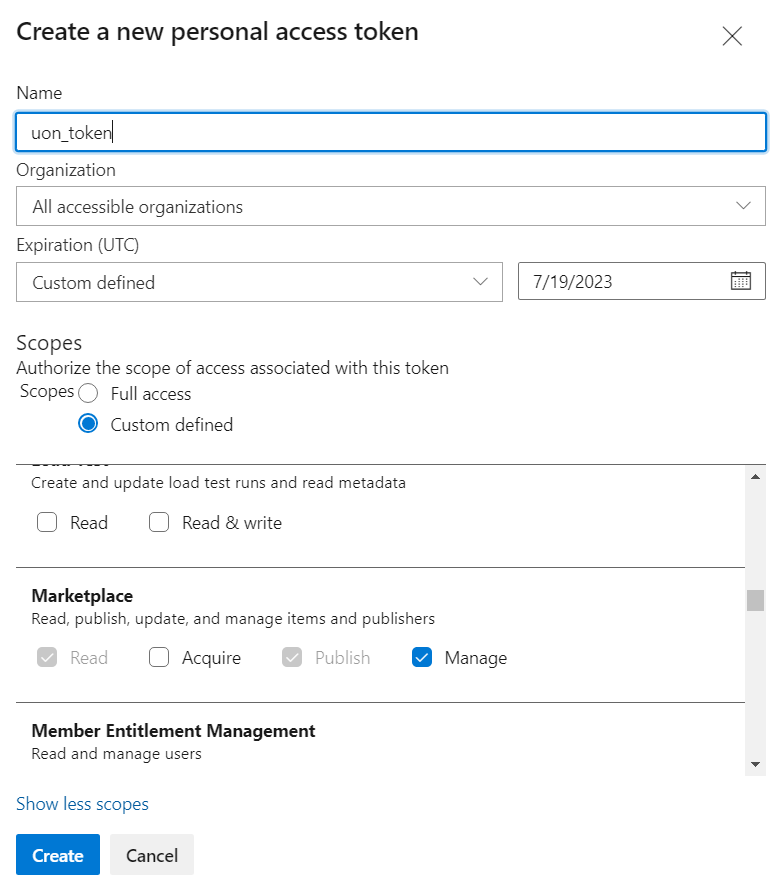
\includegraphics[width=8cm]{assets/figures/access-token.png}}
    \end{center}
    \caption[Access Token]{\label{access-token}Access Token}
\end{figure}

Ce token va nous permettre publier notre extension sur un Publisher. Celui-ci nous permettra de gérer notre extension en ligne.

Pour créer un publisher, il faut se connecter avec le même compte qui a créé l'organisation et le token ci-dessus via la \href{https://marketplace.visualstudio.com/manage/publishers/}{management page}.

Quand cela est fait, il faut ensuite ajouter la propriété "publisher" et saisir l'id de celui-ci dans le package.json de notre extension.

Puis finalement, il suffit dans un terminal les commandes suivantes :
\begin{lstlisting}[frame=single]
    vsce login [le nom du publisher]
    Vsce publish
\end{lstlisting}

\textbf{Remarque} : Attention au terminal utilisé. Le terminal de node (git.bash) ne propose pas toujours les options de sélections à l'utilisateur. Dans mon cas il était impossible de saisir le PAT et donc une erreur était affichée.

\begin{figure}[!h]
    \begin{center}
        \frame{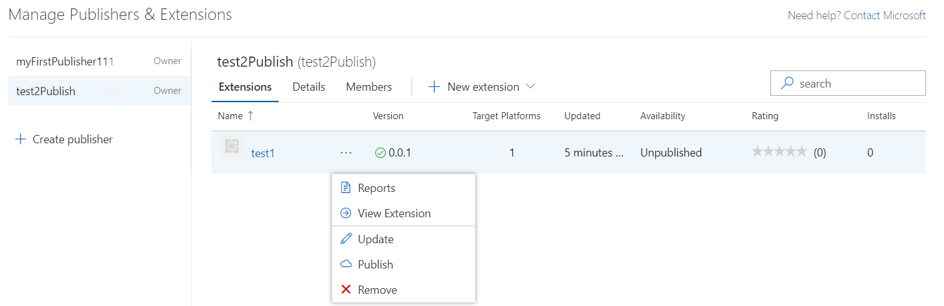
\includegraphics[width=10cm]{assets/figures/manage-publisher.png}}
    \end{center}
    \caption[Interface web pour manager l'extension]{\label{manage-publisher} Interface web pour manager l'extension}
\end{figure}

Il est ensuite facile de manager l'extension au travers de la page web.
L'extension apparaitra automatiquement dans le marketplace si elle est publiée.


\section{Génération du Parser ANTLR}
\subsubsection{Grammaire}
Le fichier de grammaire doit respecter les points suivants : \textbf{[TODO]}

\textbf{Attention} : Utiliser des majuscules pour une règle, correspond à définir un "Lexer rule" et utiliser des minuscules à un  "Parser rule".

Quand le fichier de grammaire est écrit, il suffit de lancer le code suivant :

\begin{lstlisting}[frame=single]
    antlr4ts UON.g4 -no-listener -no-visitor -o generated -Xexact-output-dir
\end{lstlisting}

Il nous génère ces fichiers :
\begin{itemize}
    \item UON.interp
    \item UON.tokens
    \item UONLexer.interp
    \item UONLexer.tokens
    \item UONLexer.ts
    \item UONParser.ts
\end{itemize}

\subsection{Arbre (CST)}

%"Notice that technically what you get from ANTLR is a parse tree rather than an AST.
% The difference is that a parse tree is exactly what comes out of the parser, while the AST is a more refined version
%of the parse tree. You create the AST by manipulating the parse tree, in order to get something that is easier to use by subsequent parts of your program"
% Citation ?

ANTLR va générer un arbre parsé. Plus précisément un CST (concrete syntax tree).
Il contient tous les noeuds de la grammaire. Certains sont superflus pour en tirer un sens.

Si on veut un AST, on doit parcouir l'arbre (avec des visiteurs ou listeners) pour en tirer un arbre plus simple.

\begin{figure}[!h]
    \begin{center}
        \frame{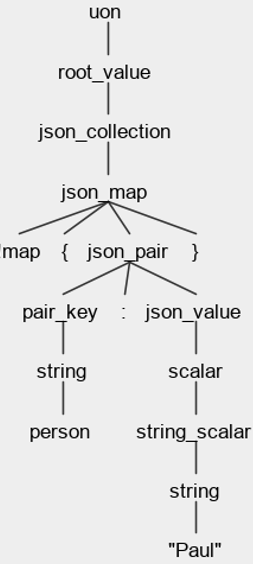
\includegraphics[width=3cm]{assets/figures/tree.png}}
    \end{center}
    \caption[UON CST]{\label{uon-tree} UON CST}
\end{figure}


\section{Syntax highlighting}

%TODO : Expliquer la stratégie pour la coloration du format json, yaml et schema, Il faudrait une explication sur les "composition"  }
%TODO : Essayer de garder une cohérence dans la couleur du texte saisi à un emplacement : exemple orange partout pour un string sauf cas particulier...
%Vérifier ça ! -> par ex. "key(description) : faux... en json et yaml"}
%TODO : key avec et sans guillemet ? Quelles règles pour une clé ? (voir grammaire originel)}
%TODO :: Approfondir explication des règles + regex (montrer des exemples ?) + Mentionner la découverte personnel dans le fichier tm : Captures + appliquer une règle à une capture spécifique}
%TODO : difficulté regex ne fonctionne pas...}

%TODO : Reserved Symbols}
% TODO : quelle couleur par défaut (gérer les entres deux) ?
% quand afficher des erreurs

La coloration syntaxique permet que chaque élément du texte soit affiché dans l'éditeur avec une coloration et un style en fonction de son type.
Il y a 2 composantes principales.
\begin{itemize}
    \item La tokenisation qui consiste à séparer le texte en une liste de token.
    \item La thémisation (Theming) qui permet d'attribuer à un token une couleur et un style.
\end{itemize}

\begin{figure}[!h]
    \begin{center}
        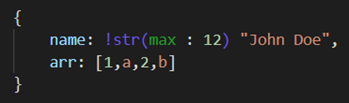
\includegraphics[width=10cm]{assets/figures/basic-uon.png}
    \end{center}
    \caption[code UON]{\label{basic-uon} Exemple basique en UON}
\end{figure}


VS code utilise Textmate grammars \cite{textmate-grammars} comme le moteur de tokénisation de la syntaxe.
Cette grammaire a été inventée par l'éditeur TextMate est a été adopté par de nombreux éditeurs et IDE.
Elle contient une liste structurée d'expressions régulières qui permet d'associer un scope à un token.
Nous définissons notre grammaire TextMate dans le fichier "uon.tmLanguage.json" qui  se trouve dans le dossier "syntax" à la racine du projet.
Ce fichier doit être référencé à travers du point de contribution "grammar" dans le package.json.

Le but de ce fichier en plus de permettre la coloration syntaxique, et qu'il permet également de rendre l'éditeur de texte "intelligent" quant au contexte dans lequel se trouve le caret. Cela permet d'avoir des comportements différents selon la situation (ex : Pas de bracket closing dans les commentaires).

\subsection{Scope}
Un scope défini le contexte du token et peut-être considéré comme son type.
TextMate fournit une liste de scope commun que de nombreux thèmes ciblent déjà et recommande de les utiliser. Ceci dans le but de permettre à notre langage d'être supporté le plus possible.
Les scopes sont souvent imbriqués et c'est le plus spécifique qui est utilisé pour le choix du thème.
Il est possible d'analyser notre code à l'aide du "Scope Inspector" pour visualiser la hiérarchie des scopes pour un token.

\begin{figure}[!h]
    \begin{center}
        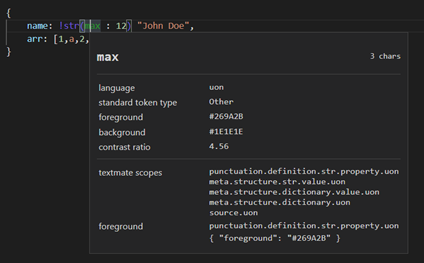
\includegraphics[width=10cm]{assets/figures/scope-inspector.png}
    \end{center}
    \caption[Scope inspector]{\label{basic-uon} Le scope inspector sur un exemple de code en UON}
\end{figure}

La section "textmate scopes" montre la liste des scopes utilisés pour le token qu'on séléctionne. Le scope le plus spécialisé se trouve au sommet.

La coloration syntaxique n'est pas considérée comme un "programmatic language feature" et donc n'est pas géré par la spécification LSP et donc l'api de VS Code non plus. Une des raisons évoquées et que ce mécanisme doit être le plus rapide possible. Et que le faire directement depuis le client garantit une latence faible.

\subsection{Stratégie concernant les noms}
Pour respecter au maximum les conventions attendues et s'assurer qu'une coloration automatique soit appliquée. La stratégie suivante a été adoptée : partir depuis un fichier de thème déjà créer (Thème dark par défaut). Et de réutiliser les scopes.

Ce fichier se trouve sur le dépôt \href{https://github.com/microsoft/vscode/blob/main/extensions/theme-defaults/themes/dark_vs.json}{suivant}.
Mais peut être également généré depuis le contrôle panel.

\subsection{Forcer le choix des couleurs}
\begin{figure}[!h]
    \begin{center}
        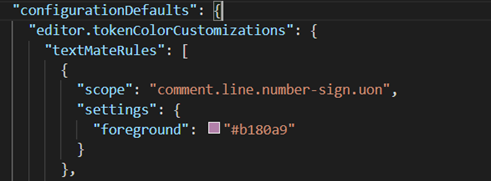
\includegraphics[width=10cm]{assets/figures/manual-settings-color.png}
    \end{center}
    \caption[Choix manuel des couleurs]{\label{manual-settings-color} Choix manuel des couleurs}
\end{figure}

On peut manuellement définir une couleur à un scope dans le fichier package.json.
Cela peut-être intéressant si aucun thème n'est associé de base à un scope.
Il est également possible de créer directement un fichier de thème.

\subsection{Fonctionnement}
\textbf{Exemple simple}

Voici ci-dessous un exemple relativement simple, mais permettant de comprendre le mécanisme général utilisé dans notre fichier "uon.tmLanguage.json" :
\begin{lstlisting}[frame=single, caption={Textmate grammar},label={Textmate grammar}]
 1  {  scopeName = 'source.untitled';
 2     patterns = (
 3        {  name = 'keyword.control.untitled';
 4           match = '\b(if|while|for|return)\b';
 5        },
 6        {  name = 'string.quoted.double.untitled';
 7           begin = '"';
 8           end = '"';
 9           patterns = (
10              {  name = 'constant.character.escape.untitled';
11                 match = '\\.';
12              }
13           );
14        },
14     );
15  }
\end{lstlisting}
\textbf{"scopeName"} (ligne 1) : Identifiant unique

\textbf{"patterns"} (ligne 2) : C'est un tableau contenant les règles actuelles utilisé pour parser le document. Elles sont appliquées dans l'ordre.
Ces règles peuvent être directement écrites à cet emplacement, mais il est aussi possible de les définir dans le "repository". Puis de les inclure.

\textbf{"repository"} : Un dictionnaire (clé-valeur) de règles.

\textbf{"name"} : Nom du scope.

Contrairement à la première règle qui ne faisait qu'un match, la deuxième définit un début et une fin sur laquelle seront appliquées les règles se trouvant dans le "patterns" suivant (à la ligne 12) . On voit qu'il est donc possible d'imbriquer les règles.

Capture : \textbf{TODO} : expliquer fonctionnement capture -> exemple "float 12 C"

Expliquer que c'est bien quand limitation clair genre {} (format json)

mais format yaml + compliqué car sur plusieurs ligne / espaces (donc juste "une ligne")
+ avoir les scalaires à la racines

arbitraire, essayer de reste cohérenet + concis
Stratégie nom... à améliorer

\subsection{Semantic Highlight}

Un point important et qu'il ne faut pas confondre la coloration syntaxique avec ce que l'on nomme la coloration sémantique. Car il s'agit d'une couche que l'éditeur rajoute sur la précédente pour l'améliorer si nécessaire.
La tokénisation sémantique permet de fournir des informations supplémentaires sur les tokens en se basant sur une compréhension profonde du langage.
De manière à résoudre les symboles dans le contexte d'un projet.

Il s'agit donc d'obtenir des informations contextualiséés afin fournir une coloration plus précise pour un token.

Par exemple avec du code Typescript :

\begin{figure}[!h]
    \begin{center}
        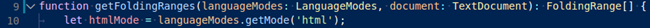
\includegraphics[width=15cm]{assets/figures/semantic-coloration-without.png}
    \end{center}
    \caption[Sans coloration sémantique]{\label{semantic-coloration-without} Sans coloration sémantique}
\end{figure}

\begin{figure}[!h]
    \begin{center}
        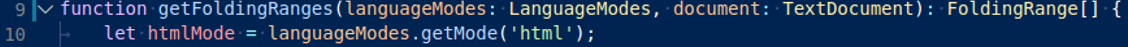
\includegraphics[width=15cm]{assets/figures/semantic-coloration-with.png}
    \end{center}
    \caption[Sans coloration sémantique ]{\label{semantic-coloration-with} Avec coloration sémantique }
\end{figure}

On voit à la ligne 10 que la colorisation de la fonction a changé et correspond maintenant à un paramètre d'une fonction.
Cela est donc intéressant pour des langages plus complexes dans leur nature qu'un langage de sérialisation. Une coloration syntaxe suffit amplement dans notre cas.
Car se baser sur la structure du document nous donne déjà toutes les informations nécessaires.

\section{Auto-completion}

Le terme "auto-complétion" existe également sous d'autres appélations (ex : autocomplétion, complétion automatique, complétion, etc.).
L'intérêt est de proposer des suggestions de saisie au fur est à mesure que l'on écrit.

\textbf{TODO : Citation}
Selon wikipédia, il s'agit d'une fonctionnalité informatique permettant à l'utilisateur de limiter la quantité d'informations qu'il saisit avec son clavier
en se voyant proposer un complément qui pourrait convenir à la chaîne de caractères qu'il a commencé à taper.

Le terme "suggestions" étant relativement vague. C'est ici ou réside la subtilité.

Il est donc nécessaire d'analyser le langage UON et de voir ce qu'il est pertinent de proposer comme suggestion de complétion.

Car en JSON ou en YAML, l'auto complétion n'existe pas vraiment du à leur nature même de ces langages de sérialisation.
Contrairement à des langages de programmation. Il n'y a pas de mots clés, on ne peut pas définir de nom de fonction, ni de classe. On ne peut également pas définir de variables.

On a donc rien de base à proposer. À la limite, seul les clé ou valeur précédement saisie peuvent éventuellement être reproposé mais cela est fait automatiquemnt sous VS Code
avec le type de complétion nommé \textbf{TODO}.

Ce comportement peut-être amélioré en utilisant par exemple "JSON-schéma" qui nous permet de définir des mots clés existants et préciser aussi leur emplacement possible.
Typiquement on peut étendre du yaml en lui spécifiant un schéma Docker est ainsi rajouter une source d'information externe.

Donc pour commencer, lorsqu'on implémente une telle fonctionnalité, il faut pouvoir répondre à une série de question :
Quelles sont les suggestions pertinentes à proposer, pourquoi et quand le faire ?

La syntaxe UON peut être exprimée par l'image suivante :

\begin{figure}[!ht]
    \begin{center}
        \frame{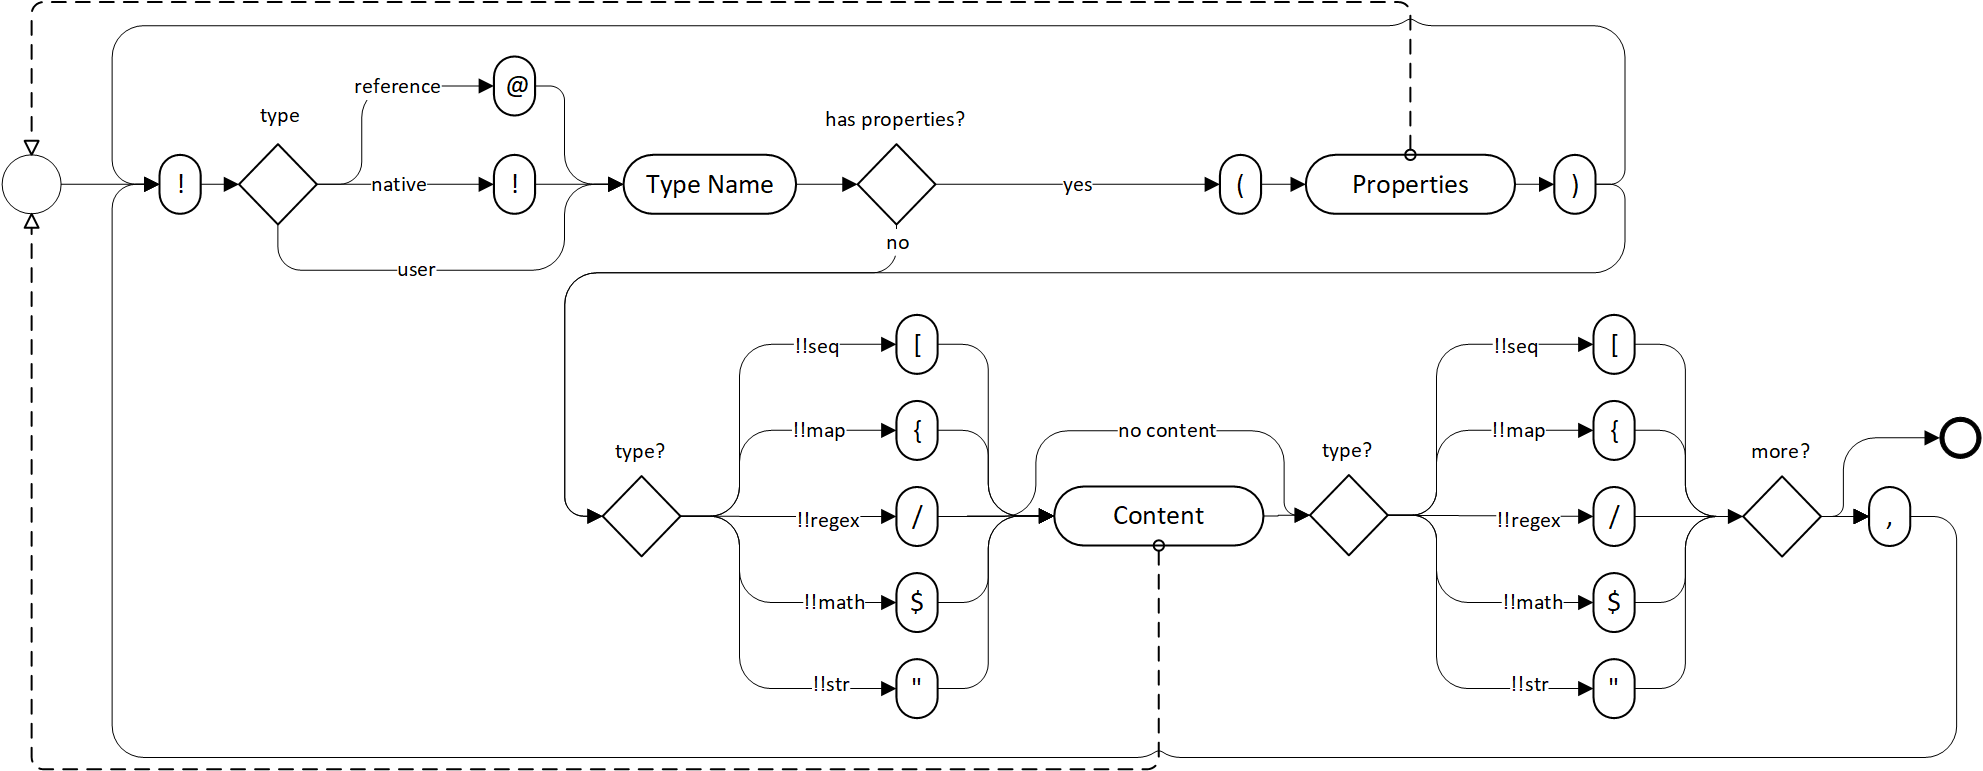
\includegraphics[width=8cm]{assets/figures/syntax.png}}
    \end{center}
    \caption[syntax]{\label{syntax} UON syntax}
\end{figure}

On n'y remarque un point extrement intéressant.

Tout est une valeur avec un type et des propriétés associés.

Les suggestions de baseront donc sur les types et leur propriétés.

%TODO : revoir c3, plus particulèrement rules et symbol tables
%    Snippet ou possible d'avoir des bloc de complétion ?}

%TODO : faire attention de bien gérer les erreurs dès que la complétions est appelé par un trigger sinon comportement aléatoire
%    ex. trigger élément qui lançait la complétion et erreur car le text parsé était faux !

%TODO : texte collé -> genre {comment:

% TODO : Se baser sur les erreurs pour essayer d'ignorer manuellement la partie avant

% Ne devrait pas afficher des proposition dans les commentaires ?

%Impossible d'avoir des suggestions si le texte est eronner : Impossible de savoir combien de token à skip + syncronisation
%"ANTL4's error strategy is to try re-synching the ATN walk to the actual input. However, that goes only so far to
%find either a single additional token or a single missing token. This won't help in this scenario,
%which would require to (theoretically) skip an unknown number of tokens and resynch."

%le moteur n'utilise pas vraiment le parser mais le toknenStream généré par le parseur.

%https://github.com/mike-lischke/antlr4-c3/issues/29


Cette fonctionnalité fait parti de ce qu'on appelle plus communément "IntelliSense" \cite{intelliSense} qui un terme général désignant diverses fonctions d'édition de code.


\subsection{antlr4-c3}

Comme mentionné au début de ce document, une approche typique pour implémenter de la complétion est d'utiliser un parser du langage.

% TODO : ERREUR avec le symbole #
Mais en complément nous allons aussi exploiter \href{https://github.com/mike-lischke/antlr4-c3}{"antlr4-c3"} (également simplement nommé c3).
Cet outil est écrit en Typescript mais existe aussi en version JAVA et C\#.
Il s'agit d'un moteur de complétion pour les parsers basés sur ANTL4. Le moteur c3 est capable de fournir des candidats de complétions.

% citation ?
Le moteur ne va pas utiliser le résultat du parse tree pour la complétion. Mais l'exécution du parser est nécessaire pour remplir le token stream sur lequelle s'appuyera le moteur.

% citation ?
\textbf{Remarque} : Le résultat du parsing n'a pas besoin d'être correcte. Il est possible de travailler avec du code incomplet ou malformé, ce qui est relativement fréquent dans un éditeur.
ANTLR4 est capable de se rétablir des erreurs et si nous utilisons le DefaultErrorStrategy nous obtiendrons un parse tree dans tous les cas.

Pourquoi un telle moteur ?

Car connaitre tout les types de tokens qu'un utilisateur serait amené à saisir ne suffit pas. Pour que la complétion soit réellement intéressante, nous voudrions connaitre quelle règle de la grammaire pourrait être valide à une position donnée.
Et cet outil apporte une solution pratique est élégante pour résoudre ce cas. %TODO source

%% todo : useless ?
%%De plus nous ne voudrions pas proposer tout ce qui est possible

Pour recevoir des candidats il suffit d'exécuter la commande suivantes.

\begin{lstlisting}[frame=single]
    let candidates = core.collectCandidates(index);
\end{lstlisting}


Nous expliquerons plus tard comment est calculé l'indice.

Nous recevorns alors un objet CandidatesCollection.

\begin{lstlisting}[frame=single]
    class CandidatesCollection {
        tokens: Map<number, TokenList>;
        rules: Map<number, RuleList>;
    }
\end{lstlisting}


On obeserve qu'en plus une liste des tokens en obtient également une liste de règles "rules".

%Tell the engine in which parser rules you are particularly interested. It will then return those to you instead of the lexer tokens they are made of.

On peut spécifier au moteur quelles règles de parseur nous intéresse. Cela nous retournera ? au lieu des tokens de lexers avec lesquels ils sont composé.

Example :


Comment aurions nous du procéder sans un tel outil ?
Il évidemment possible de le faire sans ce moteur. Un excellent article mentionne une telle implémentation aussi avec ANTLR ici.

Cela rend bien entendu le travail plus conséquent.

% todo : useless ?
%%On devrait comprendre quel type de token pourrait pourrait suivre le "caret".
%%Pour trouver ces tokens, on peut s'aider du lexer pour garder dans une liste dans les tokens trouvés dans un inputs.


\textbf{Symbol tables}

C'est un méchanisme important de c3 mais que nous n'allons pas exploiter.

Une table de symbole est une structure qui contient des informations sur des symboles, cela peut s'agir de noms, leur scopes et d'autre caractèrisiques.
Cependant, un langage de sérialisation est relativement moins complexe à gérer qu'un langage de programmation.
Nous n'avons par exemple pas à gérer des variables et leur visibilité au sein du code.

De ce fait nous n'avons alors pas besoin d'une telle source d'information complémentaire.


\textbf{Rule}

%todo


\textbf{Sorting}

%  fuzzy search algorithms to match identifiers
Pour rendre la recherche plus agréable on peut utiliser un algotihme de recheche aproximative (Fuzzy search).
% TODO

%Filtering
%Partial Matches ???? -> pas compris pourquoi il y a ce traitement si particulier ???
%Adding Heuristics
%Improving Performance


% TODO
% The ANTLR4 runtime even provides the LL1Analyzer class, which helps with retrieving follow sets for a given ATN state, but has a few shortcomings and is in general not easy to use.
% With the Code Completion Core implementation things become a lot easier. In the simplest setup you only give it a parser instance and a caret position and it will return the candidates for it. Still, a full code completion implementation requires some support code that we need to discuss first before we can come to the actual usage of the c3 engine.

% Symbol table ?

% Preferred Rules ?

% Debugging ?



Avant il n'y a avait que des solutions personnelles. Cette librairie a pour objectif de fournir une implémentation commune. Il est disponible comme node module et est écrit en Typescript.
Elle a été conçu par Mike Lischke.

% TODO
Setup basique :

\begin{lstlisting}[frame=single]
    let inputStream = new ANTLRInputStream("var c = a + b()");
    let lexer = new ExprLexer(inputStream);
    let tokenStream = new CommonTokenStream(lexer);

    let parser = new ExprParser(tokenStream);
    let errorListener = new ErrorListener();
    parser.addErrorListener(errorListener);
    let tree = parser.expression();

    let core = new c3.CodeCompletionCore(parser);
    let candidates = core.collectCandidates(0);
\end{lstlisting}

%%% TODO Explication
En ce qui concerne l'API de complétion de antlr-c3, cela ressemble un peu à ceci :

%TODO pas contractuel
\begin{lstlisting}[frame=single]
class CompletionCandidates:
    # a map of the next possible token to a list of tokens which immediately follow it,
    # if they exist (I haven't personally found any use for the following token list with my grammar)
    tokens: Mapping[TokenId, List[TokenId]]
    # a map of the current parser rule to the rule stack at that point
    rules: Mapping[RuleId, List[RuleId]]

def collect_candidates(
    parse_tree,
    ignored_tokens: List[TokenId],  # the token blacklist
    preferred_rules: List[RuleId],   # the rule whitelist
    caret_token_idx: int) -> CompletionCandidates: ...
\end{lstlisting}

% TODO https://github.com/lark-parser/lark/issues/684

% The tokens give you keyword completion and you use the rules + their contexts +
% previous parse information to do more advanced autocompletion of identifer names etc.

Of course you have to locate the caret token index yourself and you seem to end up which lots of parser rule name aliases in your grammar so they can be filtered out specifically during completion.


Nous utilisons la version 4 de ANTLR. Elle a comme avantage sur son ancienne version (ANTL3) d'avoir la structure de la grammaire directement disponible dans le parser via
un mécanisme de machine à état ATN (Augmented Transition Network). C'est ce méchanisme qui est en coeur du fonctionnement du moteur.

Dans la configuration la plus simple pour l'utiliser, il suffit de lui donner une instance du parser et une position de caret (notre curseur) pour qu'il renvoie les candidats correspondants.
Cette position est l'indice du candidat. L'explication pour le trouver se trouve dans la séction \hyperref[candidates]{\textbf{Candidats}}

On constate donc que c'est un outil relativement puissant et qui nous simplifie grandement la tâche.

\textbf{Remarque}: On pourrait penser qu'avoir à disposition un parser nous permettrait de récupérer toutes les informations nécessaires au travers d'un AST. Cependant ce n'est pas le cas pour la plupart des scénarios.
Nous pouvons savoir quels sont les tokens valide à un emplacement (ce qui est suffisant pour nous). Mais pour certains langages, des informations manquent. Par exemple des noms de classe, des objets de base de données, des membres de classes, des fonctions, etc. ne sont pas représentés dans la grammaire. 

Ci-dessous Un ATN d'une séquence :

\begin{figure}[!ht]
    \begin{center}
        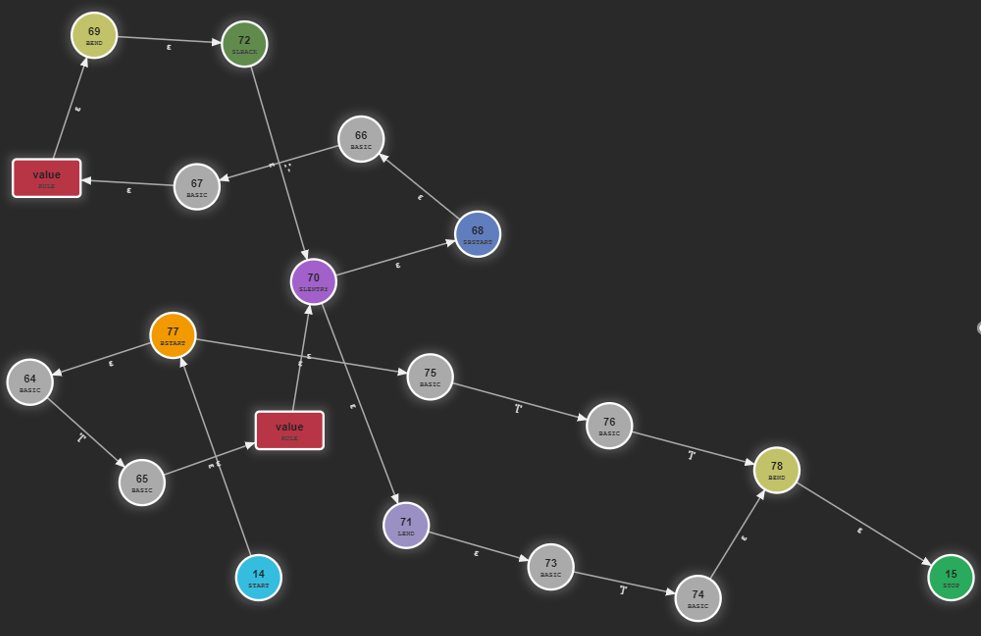
\includegraphics[width=12cm]{assets/figures/seq_ATN.png}
    \end{center}
    \caption[ATN d'une séquence]{\label{seq_ATN} ATN d'une séquence}
\end{figure}

La seule contrainte est qu'il est nécessaire que tout le code se trouvant avant le curseur soit correct. Mais ce qui se trouve à la suite peut être erroné.
Ainsi, nous pouvons revenir n'importe où dans le code, car la partie se trouvant après le curseur n'est pas prise en compte et la rédaction du code précédente est normalement correcte.
De plus, actuellement, nous n'avons pas de suggestions qui dépendraient de ce qui se trouve après le curseur.
Car par exemple dans l'exemple suivant pour du code SQL :

\begin{lstlisting}[frame=single]
SELECT | FROM USER // ("|" étant le curseur)
\end{lstlisting}

Dans ce scénario des suggestions liées à la table USER devrait être proposé et nécessiterait un traitement particulier.

Pour nous, la seule chose qui doit donc être correcte est la structure du code. C'est-à-dire que l'ordre des éléments attendus est respecté.

\subsection{Tokens ignorés}
Nous pouvons indiquer au moteur les token qui ne nous intéressent pas, pour ne pas les récupérer dans la liste des candidats.

\subsection{Tolérance}
Il semble normal que la complétion n'ait pas lieu si le code saisie est gravement erroné.
Cependant il devrait être tolérant à une certaine mesure sur des erreurs qui ne péjore pas la compréhension du code.
Une possibilité et de traiter les erreurs lors de l'analyse syntaxique, ce sujet est abordé dans la section \hyperref[error handle]{Gestion des erreurs} ci-dessous.

Mais on peut imaginer supprimer des cas potentiels d'erreurs lors de la conception de notre grammaire.
Par exemple, les erreurs sur les valeurs attendues. Une stratégie serait d'avoir un type seul qui supporterait le plus de symboles possible.
Imaginons que l'on donnerait en entrée un type incorrect à une propriété, selon la spécification officielle du langage UON.
Par exemple (max : 12a), l'erreur pourrait tout simplement ne pas exister.
Ainsi même si cela est faux syntaxiquement en UON, cela ne bloque pas le processus de l'auto-complétion.

Pour signaler à l'utilisateur que la saisie est tout de même incorrecte. On peut s'aider en parallèle de la coloration syntaxique.

\subsection{Mécanisme automatique}
VS Code va automatiquement filtrer les suggestions pendant la saisie.
Par défaut il propose également des symboles déjà existants dans le code.

\subsection{Gestion des erreurs }\label{error handle}

ANTLR à un méchanisme avancé de récupération d'erreur (Parser Error Recovery Strategy).
% TODO : centraliser les gestion d'erreur d'antlr avec celui dans le lint...
% Source...
L'idée gérnéral et d'insérer de faux token ou de supprimer les tokens non valides jusqu'à ce qu'il en trouve un qui corresponde à set de tokens connu.

% TODO : Fonctionne réelement ou je dois changer l'index aussi

On peut ajouter au parser un "ErrorListener".
Par défaut c'est la stratégie de la classe se trouvant dans le fichier \href{https://github.com/tunnelvisionlabs/antlr4ts/blob/master/src/DefaultErrorStrategy.ts}{suivant} qui est appliquée.

Mais on peut l'étendre pour redéfinir les fonctions.
Car normalement en cas d'erreur, le parser va essayé de continuer l'analyse syntaxique jusqu'à trouver un token valide.
Cependant il se peut qu'il n'y ait rien après. C'est presque tout le temps le cas lorsqu'on est en train d'écrire.
On va donc juste s'arrêter.

\subsection{Snippets}
Il est possible d'ajouter des snippets sous VS Code. C'est-à-dire des templates qui nous permettent de générer du code prédéfini. Puis de les ajouter aux suggestions.
C'est utile si à un moment donné on a le choix entre plusieurs suggestions et que l'on veut tous les avoir d'un coup.
Par exemple, on peut en UON, ajouter des attributs à un schéma :

\begin{figure}[!h]
    \begin{center}
        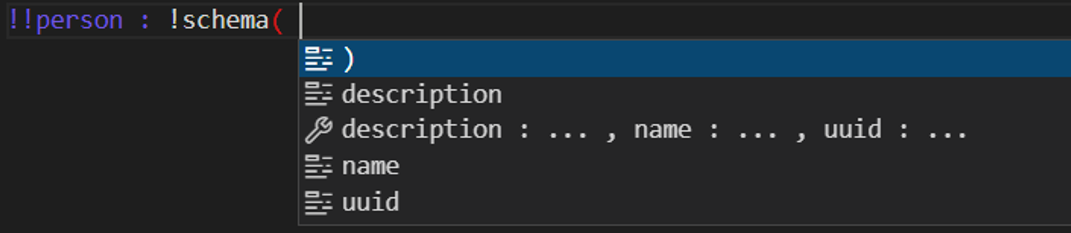
\includegraphics[width=10cm]{assets/figures/snippet-suggestion.png}
    \end{center}
    \caption[Suggestion d'un snippet]{\label{snippet-suggestion} Suggestion d'un snippet}
\end{figure}

Cependant toute la difficulté et de proposer ces suggestions au bon moment, car ne faisant pas partie du moteur de complétions d'antlr. Une idée et de se baser sur le dernier token reconnu. On pourrait ici savoir qu'il est le moment d'ajouter ce snippet, si le dernier token est de type "!schema".

\subsection{Triggers}
L'éditeur va trigger automatiquement l'autocomplétions en appelant le provider lorsque l'on saisit plusieurs caractères. Il aussi possible de l'activer manuellement en exécutant la commande "ctr + space" (par défaut).
On peut aussi ajouter au provider des symboles qui vont trigger son activation. Les symboles espace et de retour à la ligne ont été défini comme triggers, car cela semble assez naturel dans ce langage. Cependant il ne s'agit que d'une appréciation personnelle.

%TODO :
No suggestion :
quand un espace précède un nouveau mot alors c'est simple pour le placer
quand il est colé c'est + compliqué. Il faut calculer la position du début et de fin du nouveau mot car VS Code peut trigger l'autocomplete n'importe quand et du coup
avec du texte colé il peut pas savoir à partir de ou le texte en train d'etre ecrit est un mot du lnagage...mais utilité de faire ça ???

%TODO : quick-suggest-setting (par défaut ?) : https://github.com/microsoft/vscode/issues/101333}

\subsection{Candidats}\label{candidates}

Une des plus grandes diffucultés à résoudre, est d'implémenter une fonction pour convertir la positon actuelle du curseur en la position du prochain token attendu.
Pour être transmis à la fonction "collectCandidates(tokenIndex)". %todo

La documenation du projet indique bien que ce n'est pas un problème trivial à résoudre.
Un point important est de savoir si l'on tient compte ou non des espaces vides dans la grammaire.

Sans les espaces, il est difficle de gérer certains cas particuliers % TODO montrer des exemples

% TODO controler si on doit modifier l'indice ou ignorer ces tokens dans le ignore...
% TODO résoudre le cas lorsque nous rajoutons manuellement des tokens depuis le lexer
% Plus tard, nous verrons qu'il est nécessaire d'ajouter des tokens manuellement pour gérer l'indendation\dots 


Actuellement pour connaitre l'indice du ou des prochains candidats, on récupère le flux des tokens (tokenStream) trouvé lors du parsing.
Puis, on récupère dans un tableau chaque token individuellement (y compris les espaces).

Cependant lorsque l'utilisateur écrit et que cela trigger l'autocomplétion, le texte parsé est souvent incorect, car le dernier élément saisi n'est pas encore complet.

Grâce à la taille du tableau et en se basant sur les erreurs qui ont été générées, on peut déduire l'indice du ou des prochains tokens que l'on peut afficher.

\subsubsection{Index du candidat}
L'indexation est gérée de 2 manières différentes. En fonction de la prise en compte de l'espace ou non.

\begin{figure}[!h]
    \begin{center}
        \frame{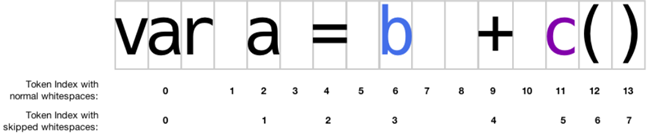
\includegraphics[width=14cm]{assets/figures/candidat-index.png}}
    \end{center}
    \caption[Indexation des candidats]{\label{candidat-index} Indexation des candidats}
\end{figure}

Cela va dépendre si on décide d'ignorer ou non les espaces dans la grammaire g4.
Les développeurs de c3 recommandent de ne pas ignorer les espaces. Car cela permet de gérer plus de cas particuliers.

%TODO : remplacer par Outline view ?}
\section{Document outlining}

%TODO : expliquer qu'on affiche pas les propriété pour l'instant ou pour toujours ?
% si pas le cas, changer strucutre pour mieux représenter les propriétés...
% Rajouter yaml

La outline view est une représentation du fichier actuellement ouvert par l'éditeur.
Les éléments peuvent être représenté de manière hiérarchique ou seulement être listés.

Un élément de l'outline (noeud) représente un élément unique du texte ou une structure.
Généralement un noeud nous permet de nous rediréger sur l'élément du fichier lorsqu'on le séléctionne.
Il faut donc pouvoir être capable de récupérer la position d'un élément du fichier.

Il est possible obtenir la structure d'un fichier en analysant manuellement le texte (par exemple ligne par ligne). Mais cette approche n'est pas optimale et il serait diffile de représenter la strucutre hiérarchique du document.

Nous allons donc utiliser notre parser.
Le résulat du parsing est un "parse tree" (aussi nommé CST) qui est une représentation concrète de notre input. Le parse tree contient toutes les infomrations et beaucoup d'entre elles ne nous intéressent pas.
Typiquement les informations grammaticales et structurelles.

\begin{figure}[!h]
    \begin{center}
        \frame{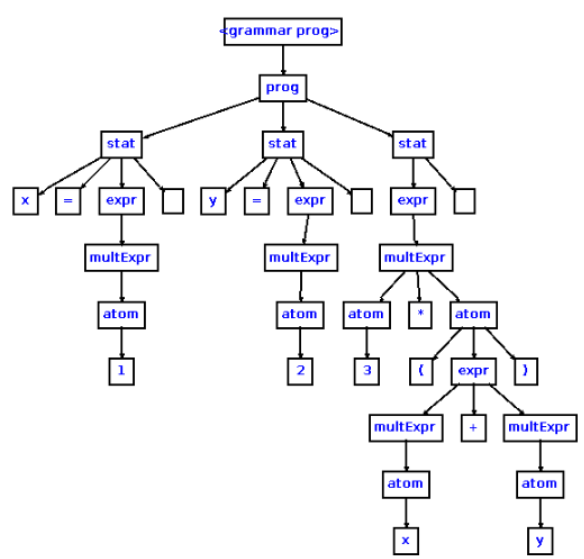
\includegraphics[width=10cm]{assets/figures/parse-tree.PNG}}
    \end{center}
    \caption[UON parse tree]{\label{parse-tree} UON parse tree}
\end{figure}

C'est pourquoi il faut pouvoir le parcourir pour en extraire un AST.
Un AST est une représentation abstraite de notre input. Il ne contient généralement que les informations les plus pertinents.

\begin{figure}[!h]
    \begin{center}
        \frame{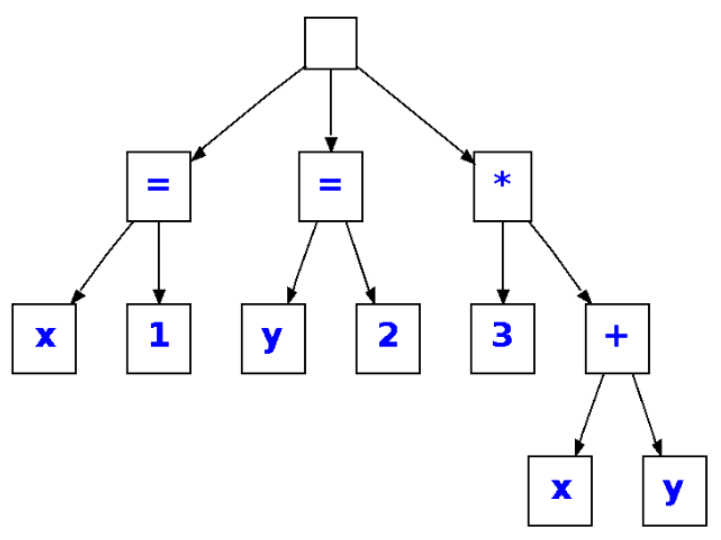
\includegraphics[width=10cm]{assets/figures/ast.PNG}}
    \end{center}
    \caption[UON AST]{\label{ast} UON AST}
\end{figure}

%TODO : Images non contractuelles

Donc pour le générer on va vouloir récupérer uniquement les informations que l'on juge pertinentes pendant le parcours.

Pour parcourir un arbre, deux approches sont possibles : Le pattern Listener ou Visitor.
La première consiste à écouter les types de noeuds traversés qui nous intéressent. Le problème et que c'est approche ne nous permet pas de manipuler un objet en cours de route, ni gérer le flux d'exécution.
Car il n'est pas possible de communiquer entre les noeuds. Cela peut être tout de même utile si l'on veut afficher la strucure de l'arbre dans un terminal par exemple.

Contrairement à la seconde apporche, qui nous permet de gérer ces 2 cas. Et c'est donc tout naturellement que cette solution a été prévilégiée.

Cependant on ne va pas d'abord créer un AST puis construire la outline view à l'aide de celui-ci.
Nous allors directement construire l'outline view à la volé, pendant le parcours du parse tree. L'outline view sera une représentation direct de notre AST.


"Both the listener and the visitor use depth-first search"

Je me suis inspiré de l'outline json et yaml pour obtenir un résultat visuel similaire.

Que devons nous visualiser dans l'outline ?

DFS permet de garder l'odre donc manipulations facilités

DocumentSymbol

class DocumentSymbol
Represents programming constructs like variables, classes, interfaces etc. that appear in a document. 
Document symbols can be hierarchical and they have two ranges: one that encloses its definition and one
that points to its most interesting range, e.g. the range of an identifier.


Dans un premier temps ne tient pas compte des popriété
rajouter ça....

pierre angulaire

\begin{figure}[!h]
    \begin{center}
        \frame{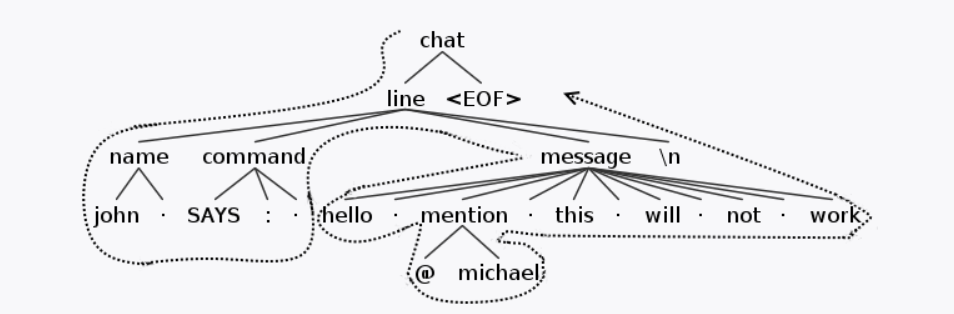
\includegraphics[width=10cm]{assets/figures/DFS.PNG}}
    \end{center}
    \caption[Algorithme de parcours en profondeur (DFS)]{\label{ast} Algorithme de parcours en profondeur (DFS)}
\end{figure}

Lors de la génération du parser, une classe Visitor a été crée et son rôle est de pouvoir retourner un élément à chaque étape du parcours.

Puis il faut ajouter le code suivant au paser \dots \textbf{TODO}

Le type de classe est générique. Et ce qui nous permet de manipuler un objet VS code \textbf{TODO : le nom} en la surchagant.
La classe surchargée est de type "any" car pendant le parcours un élément peu être de 2 natures différentes (Une valeur/terminal ou une strucutre Vscode)

%TODO : expliquer en détail

On peut avoir pendant le parcours 2 structure différentes

\subsection{La position}

Comme expliqué précédemment, il est nécessaire d'obtenir la position. Cependant nous ne possédons pas cette informations \textbf{TODO : à controler}
On va donc manipuler l'input pour obtenir le numéro de ligne en se basant sur le nombre de retour à la ligne.
Seul la ligne nous intéresse. VS code ne nous redirigant que sur celle-ci.


%TODO :TODO : parler des 2 patterns listener et visitor
%    pourquoi avoir choisi le pattern visiteurs ? https://stackoverflow.com/questions/20714492/antlr4-listeners-and-visitors-which-to-implement
%    Mentionner la provenance de la base du code (github antlr4ts) + les fichiers utilsés par le module antlrts (TreeVisitor etc...)


% visiteur explications : https://www.youtube.com/watch?v=BD-I3f0aTbs

%TODO : expliquer qu'on gènère finalement pas un AST pour l'utiliser mais qu'on crée l'arbe de symbole de manière récusrive lors du parcours (sorte d'ast directement utilisable)
%    Pas de AST car antlr génère un parsed tree qui est un arbre qui contient tout.


%TODO : ajouter figure (cst vs ast) -> Du coup quoi garder et pourquoi

%TODO : expliquer la stratégie pour récupérer la position d'un terminal

%TODO :TODO : mentionner qu'on peut avoir 5 structures (json map, json seq, yaml map, yaml seq et schema)

%TODO :
%    Quels sont les difficulté :
%    - recursion
%    - bien construire un noeud (gérer tous les cas particulier)
%    - visiteur de type any -> expliquer pourquoi j'ai fait ça : pour traiter les terminaux + les strucures...


%TODO : parler de ce qu'attend le provider (hierchical ou non, voir lsp spec)

%TODO : expliquer quelle commande lancer et pourquoi (génération des TOUS les fichiers :
%"scripts": {
%// ...
%"antlr4ts": "antlr4ts -visitor path/to/MyGrammar.g4"
%}) sinon listener et visitor ne fonctionne pas (revoir la commande fausse précédement utilisé....)


\section{Info on Hover}
% DONE : expliquer pourquoi on voulait que ça soit une feature de base / au début je pensais que ça allait être dans la grammaire ?

C'est une fonctionnalité assez triviale qui consite à afficher une explication lorsque l'on passe le curseur sur un élément.

Il s'agit donc d'une dictionnaire clé-valeur.

Cependant, même si son implémentation est relativement simple, il n'en reste pas moins un élément fortement utile et pouvant être étendu par la suite.
On pourrait le réutiliser dans la complétion pour pouvoir fournir une description d'un token dans la liste des suggestions.
Cela n'a pas été fait à cause d'une question de temps.

% TODO
%Fichier json clé-valeur....
%Intégration d'un module avec require
%utilité du dossier out / corriger bug sinon par défaut dans out/

% placement "des erreurs"
% suggestion token si possible ou expliquer qu'il faudrait redéfinir des fichiers pour récupérer le tableau ayant servi à créer le message d'erreur reçu


\section{Lint}
Un Linter est un outil d'analyse de code qui permet de détecter les erreurs et les problèmes de syntaxe.

Il est donc nécessaire de pouvoir exploiter correctement les erreurs.


On affiche les erreurs trouvé avec antlr -> avantages positions
Les erreurs sont liés au placement des tokens (manque un éléments du langages, mauvais token ou leur "ortographe").
Message trop technique mais ok pour voir d'ou viens la faute.

% https://www.antlr.org/api/Java/org/antlr/v4/runtime/ANTLRErrorStrategy.html
Antlr définit une interace pour définir une startégie concernant les erreurs recontrés durant une analyse syntaxique nommé "ANTLRErrorStrategy".
On peut distinguer trois types d'erreurs :
\begin{itemize}
    \item L'analyseur syntaxique n'a pas pu déterminer le chemin à prendre dans le ATN (aucune des alternatives disponibles ne pouvait correspondre).
    \item L'input actuel ne correspond pas ce que nous attendons.
    \item Un prédicat évalué comme faux
\end{itemize}

% TODO
Nous utiliserons le "DefaultErrorStrategy". Il a la particularité d'ignorer un token invalide pour passer au suivant.

% TODO : expliquer la classe qui nous permet de recevoir des informations en cas d'erreur
Puis on peut être notifié de ces erreurs en liant notre parser à un listener "notifyErrorListener".


% TODO
%Proposition de correction à l'aide de antlr qui nous fourni la position dans le document
%Regarder pourquoi ici on la ligne + colonne et pourquoi on pouvait pas l'avoir dans la outline view
%On utilise également une fonction et non pas un provider pour afficher les erreurs


\subsection{Suggestion}
Certains messages d'erreurs nous informes parfois des tokens qui devrait se situer à la place de celui qui a causl l'erreur.
Une idée serait donc de pouvoir remplacer ce token erronées par ceux suggérés.
Le problème et que cette information ne se trouve sous forme textuelle.
Il faudrait donc pouvoir analyser les fichiers de stratégie et les modifiers pour en récuper la liste des tokens....

% TODO surcharger des méthodes pour pouvoir être notifié des tokens manquant
\section{Fonctionnalités triviales}
Il s'agit de fonctionnalités couramment disponibles dans un support de langage. Leur implémentation est relativement simple et rapide et n'a donc pas été mentionnée dans le cahier des charges.
Les suivantes ont été implémentées :

\textbf{Comment}
\begin{itemize}
    \item Il est possible de commenter du code sous forme de ligne.
    \item Il est possible de commenter et décommenter du code (Toggling)
\end{itemize}

\textbf{Symbol pairs}
\begin{itemize}
    \item Il est possible de faire la correspondance pour certaines paires de symboles à l'aide d'une indication visuelle. (Matching)
    \item Certains symboles du langage doivent être automatiquement complétés si l'utilisateur saisit le premier élément de celle-ci. (Autoclosing)
\end{itemize}

\textbf{Code folding}
\begin{itemize}
    \item Cacher un bloc de code sur une ligne en fonction de son niveau d'indentation.
\end{itemize}

% TODO
% Couplage de fonctionnalité - logique
% Info on hover - autocompletion
% lint - code outline

\chapter{Intégration continue}

% TODO : expliquer l'architecture des fichiers test

https://code.visualstudio.com/api/working-with-extensions/testing-extension

If you are using the Yeoman Generator to scaffold an extension, integration tests are already created for you....

In the generated extension, you can use npm run test or yarn test to run the integration tests that:

Downloads and unzips latest version of VS Code.
Runs the Mocha tests specified by the extension test runner script.

use mocha api...
https://mochajs.org/api/


Expliquer les différents types de tests automatisés (unitaire, intégrations, de bout en bout)

focalisation sur les tests unitaires ?

Ce qu'on veut tester et pourquoi...

Penser au futur...extensibilité

Est-ce que tout est testable ?


\section{Autocomplétion}
% Todo : expliquer les tests
example c3, on peut tester qu'un token attendu soit le bon à un emplacemente de la
Revoir c3 pour autres types de test

\section{Syntax highlight}
% TODO
Est-il possible de faire appel au scope inspector dans visual studio ? pourquoi faire (je crois pas) ? -> tester qu'un token soit bien dans son scope
Regarder ça : https://github.com/PanAeon/vscode-tmgrammar-test
tester les expressions régulières ?


\section{Outline view}
% TODO
Comment tester la outline view ? car le code final est fortement couplé avec la logique ?
Comment savoir que le code outline est le bon....
Tester les tailles selon différent scénario
tester le noeud parent etc...


\section{Information Hover}
% TODO
Trivial ?

\section{Lint}
% TODO
Compter le nombre d'erreur et localiser leur emplacement

\section{Regex ?}
% TODO
% regex utilisé dans la grammaire g4 + tm à vérifier ?
% utilisation d'outils en ligne : ex : https://regex101.com/
% référence officielle : https://www.regular-expressions.info/


\chapter{Publication (CD ???) et maintenance}

% Parler du CD ? Ajouter notre access Token comme secret
% Ajouter le script pour déployer dans le package.json
% Installer vsce ? pourquoi ?
% Il faut s'assurer de changer la version de l'extension dans le package.json
% On ne peut pas mettre une version inférieur ou égale

% TODO : maintenance
Les explications permettant de  reprendre le projet se trouve sur le Readme à la racine du repository...

\chapter{Planning}

% TODO : Ajouter discussion de l'avancée du travail. Êtes-vous à jour ? Avez-vous pris du retard ?
% TODO : Des implémentations pas compliqué mais peu de documentation sur antlrts dans le cadre d'une extension + faut trouver comment faire en testant parfois
% TODO :
%    Difficulté :
%    Regrouper toutes les sources.
%    Grand projet personnel....
%    Analyse des resultat

\subsection{Diagramme de gantt}
Voici le diagramme de Gantt pour ce projet.
Ce diagramme sera potentiellement mis à jour durant ce semestre du fait que certaines tâches ne sont pas connues à l'avance et pour réorganiser des taches si besoin.

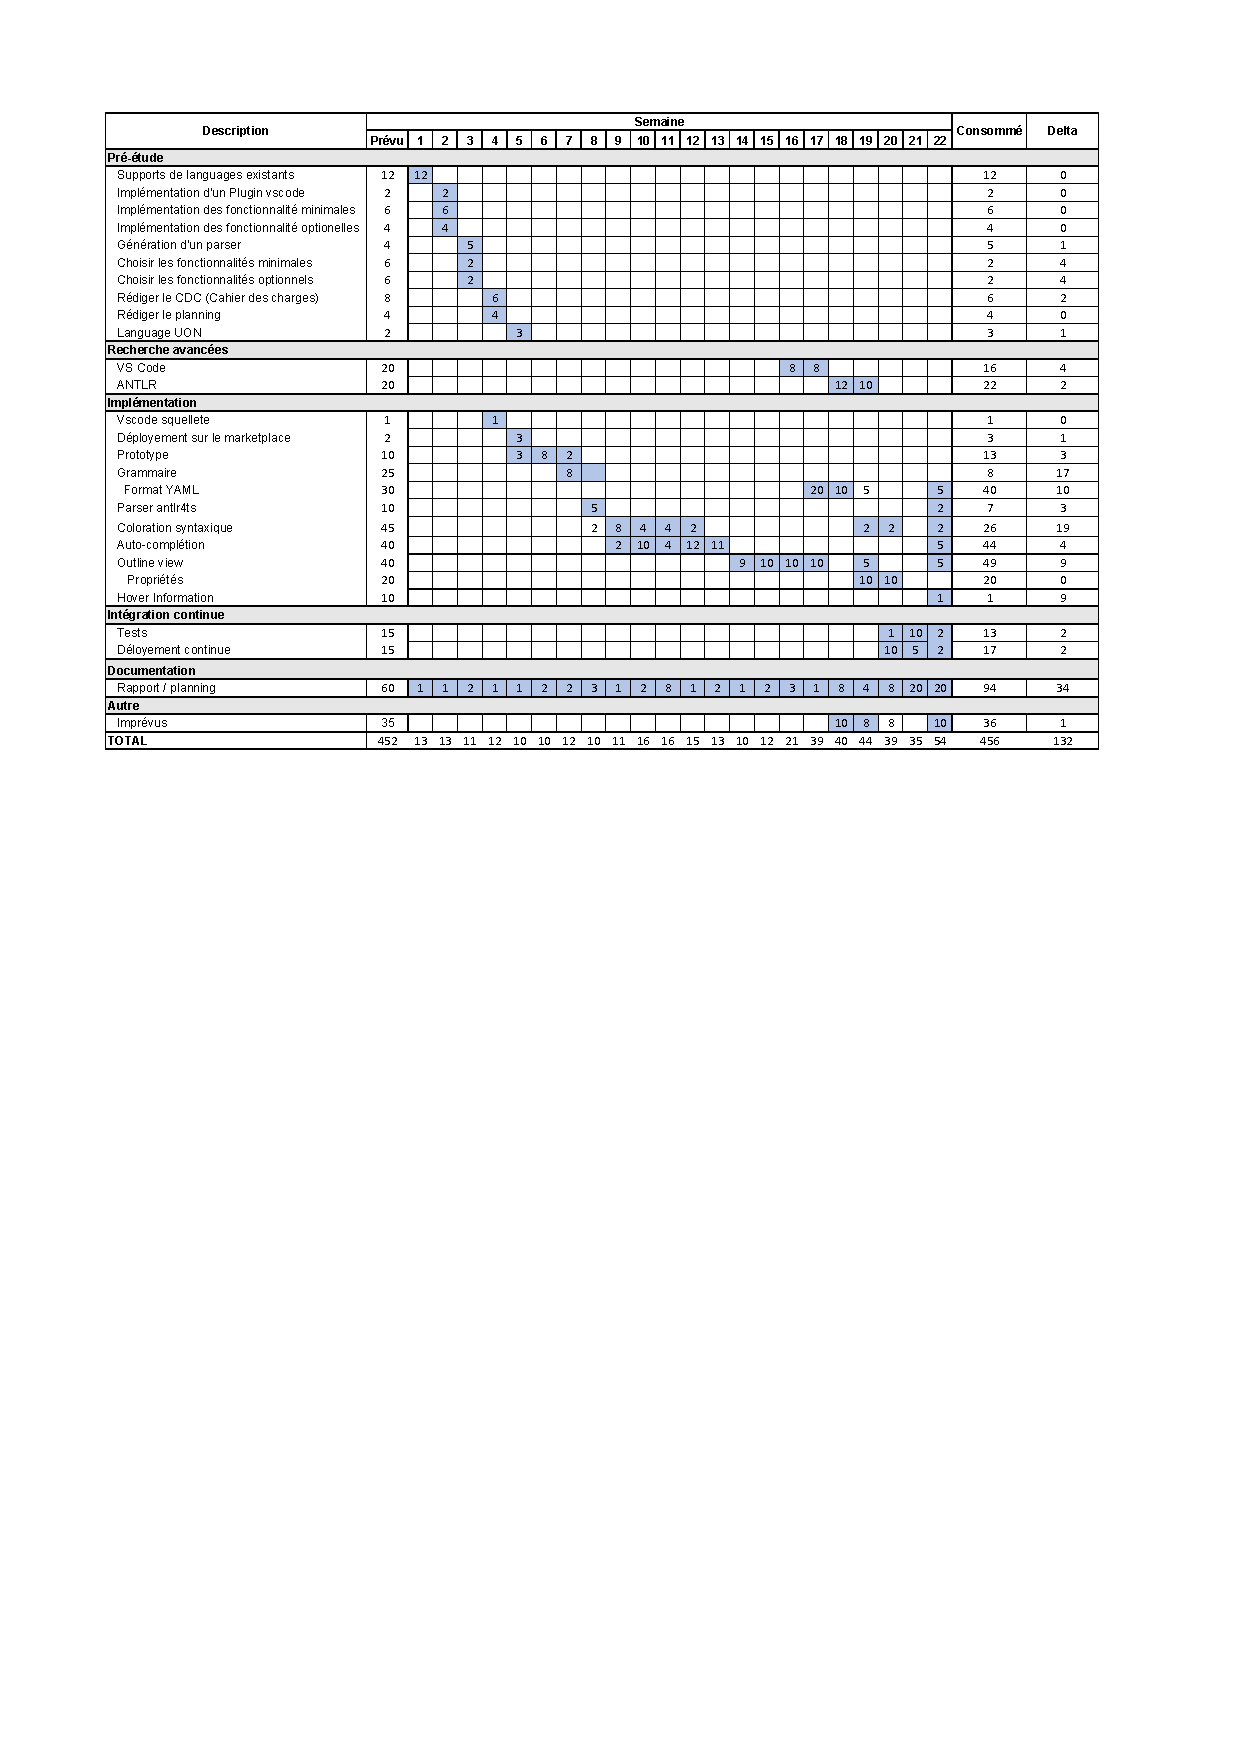
\includepdf[page=1]{assets/planning/gantt.pdf}

\chapter{Conclusion}
% TODO

\chapter{Lexique}
% TODO


%% \vfil
%% \hspace{8cm}\makeatletter\@author\makeatother\par
%% \hspace{8cm}\begin{minipage}{5cm}
%%if
% Place pour signature numérique
%%\printsignature
%%fi
%% \end{minipage}
%% \clearpage

%% \let\cleardoublepage\clearpage
%% \backmatter

%% \label{glossaire}
%% \printnoidxglossary
\textbf{TODO : Ajouter dans la Bibliographie https://www.regular-expressions.info/anchors.html}
\printbibliography
\addcontentsline{toc}{chapter}{Bibliographie}
%% \label{index}
%% \printindex

\end{document}
